\documentclass[twoside]{book}

% Packages required by doxygen
\usepackage{fixltx2e}
\usepackage{calc}
\usepackage{doxygen}
\usepackage[export]{adjustbox} % also loads graphicx
\usepackage{graphicx}
\usepackage[utf8]{inputenc}
\usepackage{makeidx}
\usepackage{multicol}
\usepackage{multirow}
\PassOptionsToPackage{warn}{textcomp}
\usepackage{textcomp}
\usepackage[nointegrals]{wasysym}
\usepackage[table]{xcolor}

% Font selection
\usepackage[T1]{fontenc}
\usepackage[scaled=.90]{helvet}
\usepackage{courier}
\usepackage{amssymb}
\usepackage{sectsty}
\renewcommand{\familydefault}{\sfdefault}
\allsectionsfont{%
  \fontseries{bc}\selectfont%
  \color{darkgray}%
}
\renewcommand{\DoxyLabelFont}{%
  \fontseries{bc}\selectfont%
  \color{darkgray}%
}
\newcommand{\+}{\discretionary{\mbox{\scriptsize$\hookleftarrow$}}{}{}}

% Page & text layout
\usepackage{geometry}
\geometry{%
  a4paper,%
  top=2.5cm,%
  bottom=2.5cm,%
  left=2.5cm,%
  right=2.5cm%
}
\tolerance=750
\hfuzz=15pt
\hbadness=750
\setlength{\emergencystretch}{15pt}
\setlength{\parindent}{0cm}
\setlength{\parskip}{0.2cm}
\makeatletter
\renewcommand{\paragraph}{%
  \@startsection{paragraph}{4}{0ex}{-1.0ex}{1.0ex}{%
    \normalfont\normalsize\bfseries\SS@parafont%
  }%
}
\renewcommand{\subparagraph}{%
  \@startsection{subparagraph}{5}{0ex}{-1.0ex}{1.0ex}{%
    \normalfont\normalsize\bfseries\SS@subparafont%
  }%
}
\makeatother

% Headers & footers
\usepackage{fancyhdr}
\pagestyle{fancyplain}
\fancyhead[LE]{\fancyplain{}{\bfseries\thepage}}
\fancyhead[CE]{\fancyplain{}{}}
\fancyhead[RE]{\fancyplain{}{\bfseries\leftmark}}
\fancyhead[LO]{\fancyplain{}{\bfseries\rightmark}}
\fancyhead[CO]{\fancyplain{}{}}
\fancyhead[RO]{\fancyplain{}{\bfseries\thepage}}
\fancyfoot[LE]{\fancyplain{}{}}
\fancyfoot[CE]{\fancyplain{}{}}
\fancyfoot[RE]{\fancyplain{}{\bfseries\scriptsize Generated by Doxygen }}
\fancyfoot[LO]{\fancyplain{}{\bfseries\scriptsize Generated by Doxygen }}
\fancyfoot[CO]{\fancyplain{}{}}
\fancyfoot[RO]{\fancyplain{}{}}
\renewcommand{\footrulewidth}{0.4pt}
\renewcommand{\chaptermark}[1]{%
  \markboth{#1}{}%
}
\renewcommand{\sectionmark}[1]{%
  \markright{\thesection\ #1}%
}

% Indices & bibliography
\usepackage{natbib}
\usepackage[titles]{tocloft}
\setcounter{tocdepth}{3}
\setcounter{secnumdepth}{5}
\makeindex

% Hyperlinks (required, but should be loaded last)
\usepackage{ifpdf}
\ifpdf
  \usepackage[pdftex,pagebackref=true]{hyperref}
\else
  \usepackage[ps2pdf,pagebackref=true]{hyperref}
\fi
\hypersetup{%
  colorlinks=true,%
  linkcolor=blue,%
  citecolor=blue,%
  unicode%
}

% Custom commands
\newcommand{\clearemptydoublepage}{%
  \newpage{\pagestyle{empty}\cleardoublepage}%
}


%===== C O N T E N T S =====

\begin{document}

% Titlepage & ToC
\hypersetup{pageanchor=false,
             bookmarks=true,
             bookmarksnumbered=true,
             pdfencoding=unicode
            }
\pagenumbering{roman}
\begin{titlepage}
\vspace*{7cm}
\begin{center}%
{\Large Software Design }\\
\vspace*{1cm}
{\large Generated by Doxygen 1.8.10}\\
\end{center}
\end{titlepage}
\clearemptydoublepage
\tableofcontents
\clearemptydoublepage
\pagenumbering{arabic}
\hypersetup{pageanchor=true}

%--- Begin generated contents ---
\chapter{Hierarchical Index}
\section{Class Hierarchy}
This inheritance list is sorted roughly, but not completely, alphabetically\+:\begin{DoxyCompactList}
\item \contentsline{section}{Control\+Data}{\pageref{structControlData}}{}
\item \contentsline{section}{Machine}{\pageref{classMachine}}{}
\begin{DoxyCompactList}
\item \contentsline{section}{Movement\+Data}{\pageref{classMovementData}}{}
\end{DoxyCompactList}
\item \contentsline{section}{Socket}{\pageref{classSocket}}{}
\begin{DoxyCompactList}
\item \contentsline{section}{Server\+Socket}{\pageref{classServerSocket}}{}
\end{DoxyCompactList}
\item thread\begin{DoxyCompactList}
\item \contentsline{section}{Worker}{\pageref{classWorker}}{}
\end{DoxyCompactList}
\end{DoxyCompactList}

\chapter{Class Index}
\section{Class List}
Here are the classes, structs, unions and interfaces with brief descriptions\+:\begin{DoxyCompactList}
\item\contentsline{section}{\hyperlink{classCLIENT}{C\+L\+I\+E\+N\+T} }{\pageref{classCLIENT}}{}
\item\contentsline{section}{\hyperlink{structControlData}{Control\+Data} }{\pageref{structControlData}}{}
\item\contentsline{section}{\hyperlink{classHoymeFloors}{Hoyme\+Floors} }{\pageref{classHoymeFloors}}{}
\item\contentsline{section}{\hyperlink{classHoymeMachines}{Hoyme\+Machines} }{\pageref{classHoymeMachines}}{}
\item\contentsline{section}{\hyperlink{classHoymeMachines2}{Hoyme\+Machines2} }{\pageref{classHoymeMachines2}}{}
\item\contentsline{section}{\hyperlink{classKittFloors}{Kitt\+Floors} }{\pageref{classKittFloors}}{}
\item\contentsline{section}{\hyperlink{classMainWindow}{Main\+Window} }{\pageref{classMainWindow}}{}
\item\contentsline{section}{\hyperlink{classServerSocket}{Server\+Socket} }{\pageref{classServerSocket}}{}
\item\contentsline{section}{\hyperlink{classSocket}{Socket} }{\pageref{classSocket}}{}
\item\contentsline{section}{\hyperlink{classWorker}{Worker} }{\pageref{classWorker}}{}
\end{DoxyCompactList}

\chapter{File Index}
\section{File List}
Here is a list of all files with brief descriptions\+:\begin{DoxyCompactList}
\item\contentsline{section}{\hyperlink{client_8cpp}{client.\+cpp} }{\pageref{client_8cpp}}{}
\item\contentsline{section}{\hyperlink{PiClasses_8cpp}{Pi\+Classes.\+cpp} }{\pageref{PiClasses_8cpp}}{}
\item\contentsline{section}{\hyperlink{PiClasses_8h}{Pi\+Classes.\+h} }{\pageref{PiClasses_8h}}{}
\item\contentsline{section}{\hyperlink{pro4_8cpp}{pro4.\+cpp} }{\pageref{pro4_8cpp}}{}
\item\contentsline{section}{\hyperlink{Socket_8cpp}{Socket.\+cpp} }{\pageref{Socket_8cpp}}{}
\item\contentsline{section}{\hyperlink{Socket_8h}{Socket.\+h} }{\pageref{Socket_8h}}{}
\item\contentsline{section}{\hyperlink{Worker_8cpp}{Worker.\+cpp} }{\pageref{Worker_8cpp}}{}
\item\contentsline{section}{\hyperlink{Worker_8h}{Worker.\+h} }{\pageref{Worker_8h}}{}
\end{DoxyCompactList}

\chapter{Class Documentation}
\hypertarget{structControlData}{}\section{Control\+Data Struct Reference}
\label{structControlData}\index{Control\+Data@{Control\+Data}}


{\ttfamily \#include $<$Worker.\+h$>$}

\subsection*{Public Member Functions}
\begin{DoxyCompactItemize}
\item 
\hyperlink{structControlData_a575219e5e0bc27904dc2aa7b1315d356}{Control\+Data} ()
\end{DoxyCompactItemize}
\subsection*{Public Attributes}
\begin{DoxyCompactItemize}
\item 
atomic$<$ int $>$ \hyperlink{structControlData_ac8fbf80345423cf5650ae64bfb10dc88}{contin}
\end{DoxyCompactItemize}


\subsection{Detailed Description}
data structure for managing control of the server 

\subsection{Constructor \& Destructor Documentation}
\hypertarget{structControlData_a575219e5e0bc27904dc2aa7b1315d356}{}\index{Control\+Data@{Control\+Data}!Control\+Data@{Control\+Data}}
\index{Control\+Data@{Control\+Data}!Control\+Data@{Control\+Data}}
\subsubsection[{Control\+Data()}]{\setlength{\rightskip}{0pt plus 5cm}Control\+Data\+::\+Control\+Data (
\begin{DoxyParamCaption}
{}
\end{DoxyParamCaption}
)\hspace{0.3cm}{\ttfamily [inline]}}\label{structControlData_a575219e5e0bc27904dc2aa7b1315d356}
default constructor \begin{DoxyParagraph}{State Changes}
assign 1 to contin 
\end{DoxyParagraph}

\begin{DoxyCode}
19 \{ \hyperlink{structControlData_ac8fbf80345423cf5650ae64bfb10dc88}{contin} = 1; \}
\end{DoxyCode}


\subsection{Member Data Documentation}
\hypertarget{structControlData_ac8fbf80345423cf5650ae64bfb10dc88}{}\index{Control\+Data@{Control\+Data}!contin@{contin}}
\index{contin@{contin}!Control\+Data@{Control\+Data}}
\subsubsection[{contin}]{\setlength{\rightskip}{0pt plus 5cm}atomic$<$int$>$ Control\+Data\+::contin}\label{structControlData_ac8fbf80345423cf5650ae64bfb10dc88}
continue serving while contin is non-\/zero. The type atomic$<$int$>$ prevents \char`\"{}race condition\char`\"{} errors if multiple threads try to access contin at the same time 

The documentation for this struct was generated from the following file\+:\begin{DoxyCompactItemize}
\item 
\hyperlink{Worker_8h}{Worker.\+h}\end{DoxyCompactItemize}

\hypertarget{classMachine}{}\section{Machine Class Reference}
\label{classMachine}\index{Machine@{Machine}}


{\ttfamily \#include $<$machine.\+h$>$}

\subsection*{Public Member Functions}
\begin{DoxyCompactItemize}
\item 
\hyperlink{classMachine_a76cfdcb722a27b8ac4c28d23b3e6212b}{Machine} (const char $\ast$Machine\+Id\+N)
\item 
int \hyperlink{classMachine_afafc49fd188ba582bdd6a0ecd714fb79}{get\+Timer} (void)
\item 
bool \hyperlink{classMachine_ab36b6edda2cbd7ae642d849eeda58a6e}{get\+Status} (void)
\item 
void \hyperlink{classMachine_a09f13c6c9a88ed77ef83ec8cfdafada3}{error\+Report} (char $\ast$email\+Id)
\item 
void \hyperlink{classMachine_aa5d8ae35383f5957bcad59226d4a44ed}{set\+Notification} (char $\ast$email\+Id)
\item 
char $\ast$ \hyperlink{classMachine_ae59177ed732c7ee3d80797310efba80d}{get\+Machine\+Id} (void)
\end{DoxyCompactItemize}
\subsection*{Private Member Functions}
\begin{DoxyCompactItemize}
\item 
int \hyperlink{classMachine_a87c0700309cbbba927df91207f29c91e}{pull\+Machine\+Id\+No} (const char $\ast$\hyperlink{classMachine_a3b65ac5d1d92eb6bb34302dea5e95260}{Machine\+Id})
\item 
char \hyperlink{classMachine_a47b70082f9d4417ae0d04b064eca7f11}{pull\+Machine\+Type} (const char $\ast$\hyperlink{classMachine_a3b65ac5d1d92eb6bb34302dea5e95260}{Machine\+Id})
\item 
char $\ast$ \hyperlink{classMachine_abb9fdde34f896ef4bd3eb7f77e3a999a}{makecopy} (const char $\ast$ch)
\end{DoxyCompactItemize}
\subsection*{Private Attributes}
\begin{DoxyCompactItemize}
\item 
char $\ast$ \hyperlink{classMachine_a3b65ac5d1d92eb6bb34302dea5e95260}{Machine\+Id}
\item 
char \hyperlink{classMachine_a30d834fcaad999f106704fdf7055156f}{Machine\+Type}
\item 
int \hyperlink{classMachine_a0bc94663d87633980e77d928adb96dad}{Machine\+Id\+No}
\item 
bool \hyperlink{classMachine_aa2bac9d075b6ceba0c90b063a9f3dd01}{status}
\item 
int \hyperlink{classMachine_a34e0ad8face9abb7206f74f421c4cb59}{timer}
\end{DoxyCompactItemize}


\subsection{Constructor \& Destructor Documentation}
\hypertarget{classMachine_a76cfdcb722a27b8ac4c28d23b3e6212b}{}\index{Machine@{Machine}!Machine@{Machine}}
\index{Machine@{Machine}!Machine@{Machine}}
\subsubsection[{Machine(const char $\ast$\+Machine\+Id\+N)}]{\setlength{\rightskip}{0pt plus 5cm}Machine\+::\+Machine (
\begin{DoxyParamCaption}
\item[{const char $\ast$}]{Machine\+Id\+N}
\end{DoxyParamCaption}
)}\label{classMachine_a76cfdcb722a27b8ac4c28d23b3e6212b}

\begin{DoxyCode}
6                                        \{
7         \hyperlink{classMachine_a3b65ac5d1d92eb6bb34302dea5e95260}{MachineId}=\hyperlink{classMachine_abb9fdde34f896ef4bd3eb7f77e3a999a}{makecopy}(MachineIdN);
8         \hyperlink{classMachine_a30d834fcaad999f106704fdf7055156f}{MachineType}=\hyperlink{classMachine_a47b70082f9d4417ae0d04b064eca7f11}{pullMachineType}(MachineIdN);
9         \hyperlink{classMachine_a0bc94663d87633980e77d928adb96dad}{MachineIdNo}=\hyperlink{classMachine_a87c0700309cbbba927df91207f29c91e}{pullMachineIdNo}(MachineIdN);
10     \}
\end{DoxyCode}


\subsection{Member Function Documentation}
\hypertarget{classMachine_a09f13c6c9a88ed77ef83ec8cfdafada3}{}\index{Machine@{Machine}!error\+Report@{error\+Report}}
\index{error\+Report@{error\+Report}!Machine@{Machine}}
\subsubsection[{error\+Report(char $\ast$email\+Id)}]{\setlength{\rightskip}{0pt plus 5cm}void Machine\+::error\+Report (
\begin{DoxyParamCaption}
\item[{char $\ast$}]{email\+Id}
\end{DoxyParamCaption}
)\hspace{0.3cm}{\ttfamily [inline]}}\label{classMachine_a09f13c6c9a88ed77ef83ec8cfdafada3}

\begin{DoxyCode}
50                                     \{
51         \textcolor{comment}{//gotta find a way to email the AC}
52     \}
\end{DoxyCode}
\hypertarget{classMachine_ae59177ed732c7ee3d80797310efba80d}{}\index{Machine@{Machine}!get\+Machine\+Id@{get\+Machine\+Id}}
\index{get\+Machine\+Id@{get\+Machine\+Id}!Machine@{Machine}}
\subsubsection[{get\+Machine\+Id(void)}]{\setlength{\rightskip}{0pt plus 5cm}char $\ast$ Machine\+::get\+Machine\+Id (
\begin{DoxyParamCaption}
\item[{void}]{}
\end{DoxyParamCaption}
)}\label{classMachine_ae59177ed732c7ee3d80797310efba80d}

\begin{DoxyCode}
12                                 \{
13         \textcolor{keywordflow}{return} \hyperlink{classMachine_a3b65ac5d1d92eb6bb34302dea5e95260}{MachineId};
14     \}
\end{DoxyCode}
\hypertarget{classMachine_ab36b6edda2cbd7ae642d849eeda58a6e}{}\index{Machine@{Machine}!get\+Status@{get\+Status}}
\index{get\+Status@{get\+Status}!Machine@{Machine}}
\subsubsection[{get\+Status(void)}]{\setlength{\rightskip}{0pt plus 5cm}bool Machine\+::get\+Status (
\begin{DoxyParamCaption}
\item[{void}]{}
\end{DoxyParamCaption}
)\hspace{0.3cm}{\ttfamily [inline]}}\label{classMachine_ab36b6edda2cbd7ae642d849eeda58a6e}

\begin{DoxyCode}
46                         \{
47         \textcolor{keywordflow}{return} 0;
48     \}
\end{DoxyCode}
\hypertarget{classMachine_afafc49fd188ba582bdd6a0ecd714fb79}{}\index{Machine@{Machine}!get\+Timer@{get\+Timer}}
\index{get\+Timer@{get\+Timer}!Machine@{Machine}}
\subsubsection[{get\+Timer(void)}]{\setlength{\rightskip}{0pt plus 5cm}int Machine\+::get\+Timer (
\begin{DoxyParamCaption}
\item[{void}]{}
\end{DoxyParamCaption}
)\hspace{0.3cm}{\ttfamily [inline]}}\label{classMachine_afafc49fd188ba582bdd6a0ecd714fb79}

\begin{DoxyCode}
41                       \{
42         \textcolor{comment}{//gets the timer from the server -- not exactly sure how this is going to happen though}
43         \textcolor{keywordflow}{return} 19;
44     \}
\end{DoxyCode}
\hypertarget{classMachine_abb9fdde34f896ef4bd3eb7f77e3a999a}{}\index{Machine@{Machine}!makecopy@{makecopy}}
\index{makecopy@{makecopy}!Machine@{Machine}}
\subsubsection[{makecopy(const char $\ast$ch)}]{\setlength{\rightskip}{0pt plus 5cm}char$\ast$ Machine\+::makecopy (
\begin{DoxyParamCaption}
\item[{const char $\ast$}]{ch}
\end{DoxyParamCaption}
)\hspace{0.3cm}{\ttfamily [inline]}, {\ttfamily [private]}}\label{classMachine_abb9fdde34f896ef4bd3eb7f77e3a999a}

\begin{DoxyCode}
28                                     \{        \textcolor{comment}{//the makecopy fuction to create copied of c style strings}
29     \textcolor{keywordtype}{char} * newchar;
30     \textcolor{keywordtype}{int} i=0;
31     \textcolor{keywordflow}{for} (i=0; ch[i]!=\textcolor{charliteral}{'\(\backslash\)0'}; i++);
32     newchar= \textcolor{keyword}{new} \textcolor{keywordtype}{char} [i+1];
33     \textcolor{keywordflow}{for}(\textcolor{keywordtype}{int} j=0; j<i+1; j++)
34         newchar[j]=ch[j];
35     \textcolor{keywordflow}{return} newchar;
36     \}
\end{DoxyCode}
\hypertarget{classMachine_a87c0700309cbbba927df91207f29c91e}{}\index{Machine@{Machine}!pull\+Machine\+Id\+No@{pull\+Machine\+Id\+No}}
\index{pull\+Machine\+Id\+No@{pull\+Machine\+Id\+No}!Machine@{Machine}}
\subsubsection[{pull\+Machine\+Id\+No(const char $\ast$\+Machine\+Id)}]{\setlength{\rightskip}{0pt plus 5cm}int Machine\+::pull\+Machine\+Id\+No (
\begin{DoxyParamCaption}
\item[{const char $\ast$}]{Machine\+Id}
\end{DoxyParamCaption}
)\hspace{0.3cm}{\ttfamily [inline]}, {\ttfamily [private]}}\label{classMachine_a87c0700309cbbba927df91207f29c91e}
integer that stores the value of number shown in machine\textquotesingle{}s timer 
\begin{DoxyCode}
14                                                \{
15     \textcolor{keywordtype}{char} num[4];
16     \textcolor{keywordflow}{for} (\textcolor{keywordtype}{int} i=7; i<10; i++)
17         num[i-7]=\hyperlink{classMachine_a3b65ac5d1d92eb6bb34302dea5e95260}{MachineId}[i];
18     num[3]=\textcolor{charliteral}{'\(\backslash\)0'};
19     stringstream convert(num); 
20     \textcolor{keywordtype}{int} r;
21     convert>>r;
22     \textcolor{keywordflow}{return} r;  \textcolor{comment}{//int r<<stringstream(num)}
23     \}
\end{DoxyCode}
\hypertarget{classMachine_a47b70082f9d4417ae0d04b064eca7f11}{}\index{Machine@{Machine}!pull\+Machine\+Type@{pull\+Machine\+Type}}
\index{pull\+Machine\+Type@{pull\+Machine\+Type}!Machine@{Machine}}
\subsubsection[{pull\+Machine\+Type(const char $\ast$\+Machine\+Id)}]{\setlength{\rightskip}{0pt plus 5cm}char Machine\+::pull\+Machine\+Type (
\begin{DoxyParamCaption}
\item[{const char $\ast$}]{Machine\+Id}
\end{DoxyParamCaption}
)\hspace{0.3cm}{\ttfamily [inline]}, {\ttfamily [private]}}\label{classMachine_a47b70082f9d4417ae0d04b064eca7f11}

\begin{DoxyCode}
24                                                 \{
25     \textcolor{keywordflow}{return} \hyperlink{classMachine_a3b65ac5d1d92eb6bb34302dea5e95260}{MachineId}[11];           \textcolor{comment}{//ell-12-145-l}
26     \}
\end{DoxyCode}
\hypertarget{classMachine_aa5d8ae35383f5957bcad59226d4a44ed}{}\index{Machine@{Machine}!set\+Notification@{set\+Notification}}
\index{set\+Notification@{set\+Notification}!Machine@{Machine}}
\subsubsection[{set\+Notification(char $\ast$email\+Id)}]{\setlength{\rightskip}{0pt plus 5cm}void Machine\+::set\+Notification (
\begin{DoxyParamCaption}
\item[{char $\ast$}]{email\+Id}
\end{DoxyParamCaption}
)\hspace{0.3cm}{\ttfamily [inline]}}\label{classMachine_aa5d8ae35383f5957bcad59226d4a44ed}

\begin{DoxyCode}
54                                         \{
55         \textcolor{comment}{//gotta find a way to email the user}
56     \}
\end{DoxyCode}


\subsection{Member Data Documentation}
\hypertarget{classMachine_a3b65ac5d1d92eb6bb34302dea5e95260}{}\index{Machine@{Machine}!Machine\+Id@{Machine\+Id}}
\index{Machine\+Id@{Machine\+Id}!Machine@{Machine}}
\subsubsection[{Machine\+Id}]{\setlength{\rightskip}{0pt plus 5cm}char$\ast$ Machine\+::\+Machine\+Id\hspace{0.3cm}{\ttfamily [private]}}\label{classMachine_a3b65ac5d1d92eb6bb34302dea5e95260}
\hypertarget{classMachine_a0bc94663d87633980e77d928adb96dad}{}\index{Machine@{Machine}!Machine\+Id\+No@{Machine\+Id\+No}}
\index{Machine\+Id\+No@{Machine\+Id\+No}!Machine@{Machine}}
\subsubsection[{Machine\+Id\+No}]{\setlength{\rightskip}{0pt plus 5cm}int Machine\+::\+Machine\+Id\+No\hspace{0.3cm}{\ttfamily [private]}}\label{classMachine_a0bc94663d87633980e77d928adb96dad}
Type of machine, in the id, the last letter denotes it \hypertarget{classMachine_a30d834fcaad999f106704fdf7055156f}{}\index{Machine@{Machine}!Machine\+Type@{Machine\+Type}}
\index{Machine\+Type@{Machine\+Type}!Machine@{Machine}}
\subsubsection[{Machine\+Type}]{\setlength{\rightskip}{0pt plus 5cm}char Machine\+::\+Machine\+Type\hspace{0.3cm}{\ttfamily [private]}}\label{classMachine_a30d834fcaad999f106704fdf7055156f}
The complete I\+D representing the machine ex. ell-\/2-\/123l \hypertarget{classMachine_aa2bac9d075b6ceba0c90b063a9f3dd01}{}\index{Machine@{Machine}!status@{status}}
\index{status@{status}!Machine@{Machine}}
\subsubsection[{status}]{\setlength{\rightskip}{0pt plus 5cm}bool Machine\+::status\hspace{0.3cm}{\ttfamily [private]}}\label{classMachine_aa2bac9d075b6ceba0c90b063a9f3dd01}
Id number of machine, in the complete id, the numbers in last term denote it \hypertarget{classMachine_a34e0ad8face9abb7206f74f421c4cb59}{}\index{Machine@{Machine}!timer@{timer}}
\index{timer@{timer}!Machine@{Machine}}
\subsubsection[{timer}]{\setlength{\rightskip}{0pt plus 5cm}int Machine\+::timer\hspace{0.3cm}{\ttfamily [private]}}\label{classMachine_a34e0ad8face9abb7206f74f421c4cb59}


The documentation for this class was generated from the following files\+:\begin{DoxyCompactItemize}
\item 
\hyperlink{machine_8h}{machine.\+h}\item 
\hyperlink{machine_8cpp}{machine.\+cpp}\end{DoxyCompactItemize}

\hypertarget{classMovementData}{}\section{Movement\+Data Class Reference}
\label{classMovementData}\index{Movement\+Data@{Movement\+Data}}


{\ttfamily \#include $<$Pi\+Classes.\+h$>$}

Inheritance diagram for Movement\+Data\+:\begin{figure}[H]
\begin{center}
\leavevmode
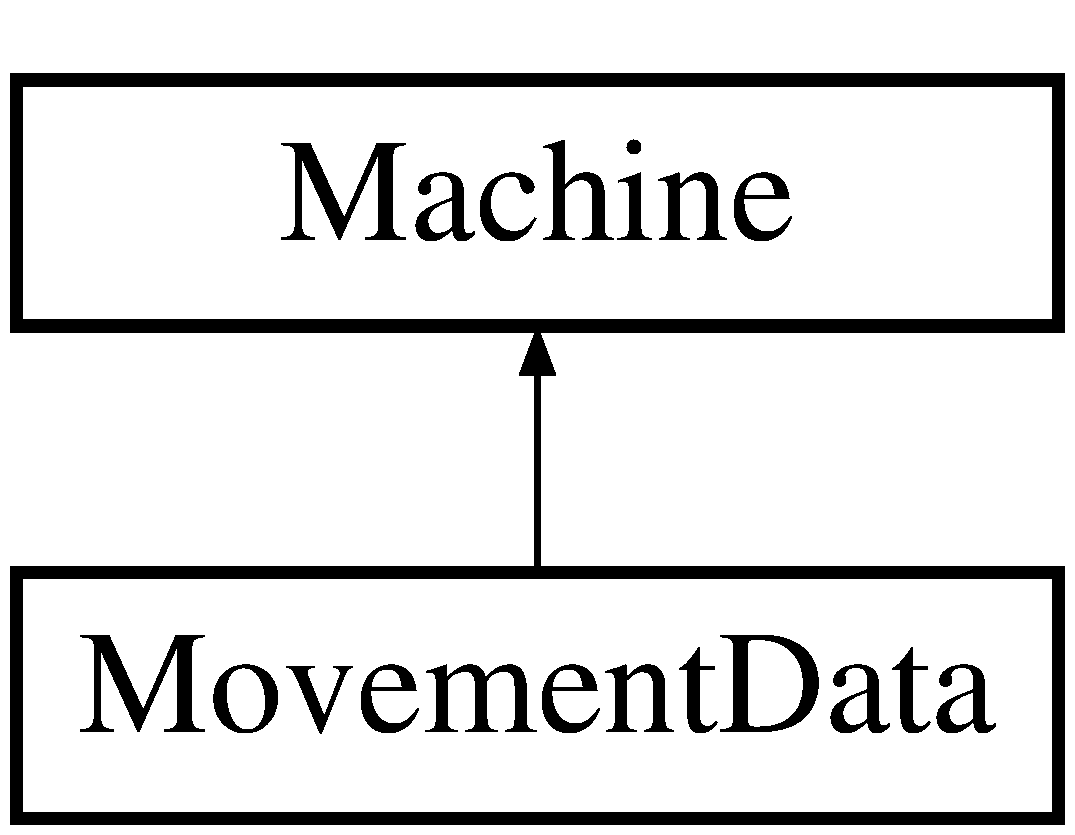
\includegraphics[height=2.000000cm]{classMovementData}
\end{center}
\end{figure}
\subsection*{Public Member Functions}
\begin{DoxyCompactItemize}
\item 
\hyperlink{classMovementData_a0592d4c39f84928dfa2a27aba5851aaf}{Movement\+Data} (void)
\item 
bool \hyperlink{classMovementData_a0460eb813078fc9e9eef646bb495a8a3}{cont\+Vib\+Check} (istream \&file)
\end{DoxyCompactItemize}
\subsection*{Static Public Attributes}
\begin{DoxyCompactItemize}
\item 
static int \hyperlink{classMovementData_abd2ebde61b24ecee8634bc0ad5a9d79c}{C\+Y\+C\+L\+E\+D\+U\+R\+A\+T\+I\+O\+N} = 2 $\ast$ 60
\end{DoxyCompactItemize}
\subsection*{Private Attributes}
\begin{DoxyCompactItemize}
\item 
int \hyperlink{classMovementData_a8bd69fc477e461a1adee4cfa8762817b}{x} \mbox{[}2\mbox{]}
\item 
int \hyperlink{classMovementData_afefc24b91fda0633c33b916eb70a9177}{y} \mbox{[}2\mbox{]}
\item 
int \hyperlink{classMovementData_a319111ec5eb9f0adc4eda7e177e8eccd}{z} \mbox{[}2\mbox{]}
\end{DoxyCompactItemize}
\subsection*{Static Private Attributes}
\begin{DoxyCompactItemize}
\item 
static int \hyperlink{classMovementData_ac6c923b8f994f87231ec00efe4393333}{T\+E\+S\+T\+T\+I\+M\+E} = 10
\end{DoxyCompactItemize}


\subsection{Detailed Description}
inherited class of \hyperlink{classMachine}{Machine} class that deals with data from the sensor 

\subsection{Constructor \& Destructor Documentation}
\hypertarget{classMovementData_a0592d4c39f84928dfa2a27aba5851aaf}{}\index{Movement\+Data@{Movement\+Data}!Movement\+Data@{Movement\+Data}}
\index{Movement\+Data@{Movement\+Data}!Movement\+Data@{Movement\+Data}}
\subsubsection[{Movement\+Data(void)}]{\setlength{\rightskip}{0pt plus 5cm}Movement\+Data\+::\+Movement\+Data (
\begin{DoxyParamCaption}
\item[{void}]{}
\end{DoxyParamCaption}
)}\label{classMovementData_a0592d4c39f84928dfa2a27aba5851aaf}
static int to store the time in seconds for reading data pattern Constructor 
\begin{DoxyCode}
36                                : \hyperlink{classMachine_a80c3b107d589a615ff42f760a5d64b32}{Machine}() \{
37   \textcolor{comment}{// MovementData::MovementData(void): Machine() \{}
38   fill\_n(\hyperlink{classMovementData_a8bd69fc477e461a1adee4cfa8762817b}{x}, 2, 0);
39   fill\_n(\hyperlink{classMovementData_afefc24b91fda0633c33b916eb70a9177}{y}, 2, 0);
40   fill\_n(\hyperlink{classMovementData_a319111ec5eb9f0adc4eda7e177e8eccd}{z}, 2, 0);
41 \}
\end{DoxyCode}


\subsection{Member Function Documentation}
\hypertarget{classMovementData_a0460eb813078fc9e9eef646bb495a8a3}{}\index{Movement\+Data@{Movement\+Data}!cont\+Vib\+Check@{cont\+Vib\+Check}}
\index{cont\+Vib\+Check@{cont\+Vib\+Check}!Movement\+Data@{Movement\+Data}}
\subsubsection[{cont\+Vib\+Check(istream \&file)}]{\setlength{\rightskip}{0pt plus 5cm}bool Movement\+Data\+::cont\+Vib\+Check (
\begin{DoxyParamCaption}
\item[{istream \&}]{file}
\end{DoxyParamCaption}
)}\label{classMovementData_a0460eb813078fc9e9eef646bb495a8a3}
method that checks the vibration pattern and analyzes it to decide if the machine\textquotesingle{}s vibration is continuous 
\begin{DoxyParams}{Parameters}
{\em reference} & to istream that represnts the address of serial port created by arduino \\
\hline
\end{DoxyParams}

\begin{DoxyCode}
46                                              \{
47   \textcolor{keywordtype}{string} data;
48   \textcolor{keywordtype}{double} startTime = \hyperlink{classMachine_a2fb11e330fa5e2b6a7134ee55ac7ef43}{getCurrentTime}();
49   \textcolor{keywordtype}{float} duration = 0;
50   \textcolor{keywordtype}{int} i = 0;
51   \textcolor{keywordtype}{int} vibct = 0;
52   \textcolor{keywordflow}{while} (duration < \hyperlink{classMovementData_ac6c923b8f994f87231ec00efe4393333}{TESTTIME}) \{
53     duration = \hyperlink{classMachine_a2fb11e330fa5e2b6a7134ee55ac7ef43}{getCurrentTime}() - startTime;
54     cout << duration << endl;
55     getline(file, data);
56     sleep(0.8f);
57     \textcolor{comment}{// MovementData::AddData(data);}
58     \textcolor{comment}{// cout<<data<<endl;}
59     \hyperlink{classMovementData_a8bd69fc477e461a1adee4cfa8762817b}{x}[0] = \hyperlink{classMovementData_a8bd69fc477e461a1adee4cfa8762817b}{x}[1];
60     \hyperlink{classMovementData_afefc24b91fda0633c33b916eb70a9177}{y}[0] = \hyperlink{classMovementData_afefc24b91fda0633c33b916eb70a9177}{y}[1];
61     \hyperlink{classMovementData_a319111ec5eb9f0adc4eda7e177e8eccd}{z}[0] = \hyperlink{classMovementData_a319111ec5eb9f0adc4eda7e177e8eccd}{z}[1];
62     \textcolor{keywordflow}{if} (data.length() == 11) \{
63       stringstream(data.substr(0, 3)) >> \hyperlink{classMovementData_a8bd69fc477e461a1adee4cfa8762817b}{x}[1];
64       stringstream(data.substr(4, 3)) >> \hyperlink{classMovementData_afefc24b91fda0633c33b916eb70a9177}{y}[1];
65       stringstream(data.substr(8, 3)) >> \hyperlink{classMovementData_a319111ec5eb9f0adc4eda7e177e8eccd}{z}[1];
66     \}
67 
68     \textcolor{keywordflow}{if} (\hyperlink{classMovementData_a8bd69fc477e461a1adee4cfa8762817b}{x}[0] < \hyperlink{classMovementData_a8bd69fc477e461a1adee4cfa8762817b}{x}[1] - 2 || \hyperlink{classMovementData_a8bd69fc477e461a1adee4cfa8762817b}{x}[0] > \hyperlink{classMovementData_a8bd69fc477e461a1adee4cfa8762817b}{x}[1] + 2 || \hyperlink{classMovementData_afefc24b91fda0633c33b916eb70a9177}{y}[0] < \hyperlink{classMovementData_afefc24b91fda0633c33b916eb70a9177}{y}[1] - 2 ||
69         \hyperlink{classMovementData_afefc24b91fda0633c33b916eb70a9177}{y}[0] > \hyperlink{classMovementData_afefc24b91fda0633c33b916eb70a9177}{y}[1] + 2 || \hyperlink{classMovementData_a319111ec5eb9f0adc4eda7e177e8eccd}{z}[0] < \hyperlink{classMovementData_a319111ec5eb9f0adc4eda7e177e8eccd}{z}[1] - 2 || \hyperlink{classMovementData_a319111ec5eb9f0adc4eda7e177e8eccd}{z}[0] > \hyperlink{classMovementData_a319111ec5eb9f0adc4eda7e177e8eccd}{z}[1] + 2) \{
70       i++;
71       vibct++;
72       cout << \textcolor{stringliteral}{"motion detected"} << endl;
73     \} \textcolor{keywordflow}{else}
74       i++;
75     \textcolor{comment}{// cout<<"not moving"<<endl;}
76   \}
77   \textcolor{keywordflow}{if} (((\textcolor{keywordtype}{float})vibct/(\textcolor{keywordtype}{float})i)>0.25)\{
78     \textcolor{keywordflow}{return} 1;
79   \} \textcolor{keywordflow}{else} \{
80     \textcolor{keywordflow}{return} 0;
81   \}
82 \}
\end{DoxyCode}


\subsection{Member Data Documentation}
\hypertarget{classMovementData_abd2ebde61b24ecee8634bc0ad5a9d79c}{}\index{Movement\+Data@{Movement\+Data}!C\+Y\+C\+L\+E\+D\+U\+R\+A\+T\+I\+O\+N@{C\+Y\+C\+L\+E\+D\+U\+R\+A\+T\+I\+O\+N}}
\index{C\+Y\+C\+L\+E\+D\+U\+R\+A\+T\+I\+O\+N@{C\+Y\+C\+L\+E\+D\+U\+R\+A\+T\+I\+O\+N}!Movement\+Data@{Movement\+Data}}
\subsubsection[{C\+Y\+C\+L\+E\+D\+U\+R\+A\+T\+I\+O\+N}]{\setlength{\rightskip}{0pt plus 5cm}int Movement\+Data\+::\+C\+Y\+C\+L\+E\+D\+U\+R\+A\+T\+I\+O\+N = 2 $\ast$ 60\hspace{0.3cm}{\ttfamily [static]}}\label{classMovementData_abd2ebde61b24ecee8634bc0ad5a9d79c}
\hypertarget{classMovementData_ac6c923b8f994f87231ec00efe4393333}{}\index{Movement\+Data@{Movement\+Data}!T\+E\+S\+T\+T\+I\+M\+E@{T\+E\+S\+T\+T\+I\+M\+E}}
\index{T\+E\+S\+T\+T\+I\+M\+E@{T\+E\+S\+T\+T\+I\+M\+E}!Movement\+Data@{Movement\+Data}}
\subsubsection[{T\+E\+S\+T\+T\+I\+M\+E}]{\setlength{\rightskip}{0pt plus 5cm}int Movement\+Data\+::\+T\+E\+S\+T\+T\+I\+M\+E = 10\hspace{0.3cm}{\ttfamily [static]}, {\ttfamily [private]}}\label{classMovementData_ac6c923b8f994f87231ec00efe4393333}
stores the values of movement on z-\/ drection at that instant \hypertarget{classMovementData_a8bd69fc477e461a1adee4cfa8762817b}{}\index{Movement\+Data@{Movement\+Data}!x@{x}}
\index{x@{x}!Movement\+Data@{Movement\+Data}}
\subsubsection[{x}]{\setlength{\rightskip}{0pt plus 5cm}int Movement\+Data\+::x\mbox{[}2\mbox{]}\hspace{0.3cm}{\ttfamily [private]}}\label{classMovementData_a8bd69fc477e461a1adee4cfa8762817b}
\hypertarget{classMovementData_afefc24b91fda0633c33b916eb70a9177}{}\index{Movement\+Data@{Movement\+Data}!y@{y}}
\index{y@{y}!Movement\+Data@{Movement\+Data}}
\subsubsection[{y}]{\setlength{\rightskip}{0pt plus 5cm}int Movement\+Data\+::y\mbox{[}2\mbox{]}\hspace{0.3cm}{\ttfamily [private]}}\label{classMovementData_afefc24b91fda0633c33b916eb70a9177}
stores the values of movement on x-\/ drection at that instant \hypertarget{classMovementData_a319111ec5eb9f0adc4eda7e177e8eccd}{}\index{Movement\+Data@{Movement\+Data}!z@{z}}
\index{z@{z}!Movement\+Data@{Movement\+Data}}
\subsubsection[{z}]{\setlength{\rightskip}{0pt plus 5cm}int Movement\+Data\+::z\mbox{[}2\mbox{]}\hspace{0.3cm}{\ttfamily [private]}}\label{classMovementData_a319111ec5eb9f0adc4eda7e177e8eccd}
stores the values of movement on y-\/ drection at that instant 

The documentation for this class was generated from the following files\+:\begin{DoxyCompactItemize}
\item 
\hyperlink{PiClasses_8h}{Pi\+Classes.\+h}\item 
\hyperlink{PiClasses_8cpp}{Pi\+Classes.\+cpp}\end{DoxyCompactItemize}

\hypertarget{classServerSocket}{}\section{Server\+Socket Class Reference}
\label{classServerSocket}\index{Server\+Socket@{Server\+Socket}}


{\ttfamily \#include $<$Socket.\+h$>$}

Inheritance diagram for Server\+Socket\+:\begin{figure}[H]
\begin{center}
\leavevmode
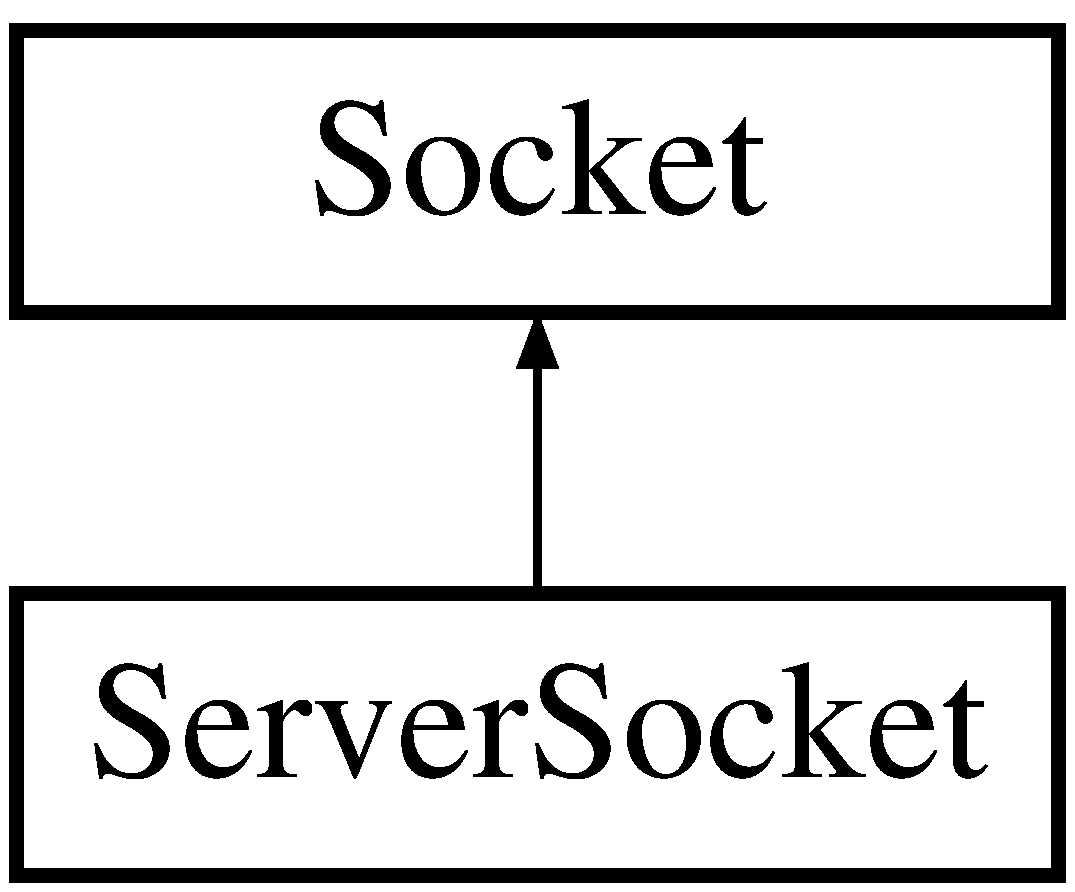
\includegraphics[height=2.000000cm]{classServerSocket}
\end{center}
\end{figure}
\subsection*{Public Member Functions}
\begin{DoxyCompactItemize}
\item 
\hyperlink{classServerSocket_a2b3098589541243241ca25495155186c}{Server\+Socket} ()
\item 
\hyperlink{classServerSocket_a3dc1a31f740e4a8d69ae10c5dcb547d6}{Server\+Socket} (int port)
\item 
int \hyperlink{classServerSocket_a6cd7ad5bd162805cb4fa9f126205e046}{bind} (int port)
\item 
\hyperlink{classSocket}{Socket} $\ast$ \hyperlink{classServerSocket_accc3d56d42aa50a5f3c920cf0b26959b}{accept} ()
\item 
int \hyperlink{classServerSocket_a3eac38fb0cc7686f758f1bc77e1b1f6b}{get\+Bound} ()
\end{DoxyCompactItemize}
\subsection*{Protected Attributes}
\begin{DoxyCompactItemize}
\item 
int \hyperlink{classServerSocket_ae7e043fe5c2a7abdcc3d83219fe5106f}{bound}
\end{DoxyCompactItemize}
\subsection*{Additional Inherited Members}


\subsection{Constructor \& Destructor Documentation}
\hypertarget{classServerSocket_a2b3098589541243241ca25495155186c}{}\index{Server\+Socket@{Server\+Socket}!Server\+Socket@{Server\+Socket}}
\index{Server\+Socket@{Server\+Socket}!Server\+Socket@{Server\+Socket}}
\subsubsection[{Server\+Socket()}]{\setlength{\rightskip}{0pt plus 5cm}Server\+Socket\+::\+Server\+Socket (
\begin{DoxyParamCaption}
{}
\end{DoxyParamCaption}
)\hspace{0.3cm}{\ttfamily [inline]}}\label{classServerSocket_a2b3098589541243241ca25495155186c}

\begin{DoxyCode}
62 : \hyperlink{classSocket_a93c96fe7bea2fc834c88786629fa041e}{Socket}() \{ \hyperlink{classServerSocket_ae7e043fe5c2a7abdcc3d83219fe5106f}{bound} = 0; \}
\end{DoxyCode}
\hypertarget{classServerSocket_a3dc1a31f740e4a8d69ae10c5dcb547d6}{}\index{Server\+Socket@{Server\+Socket}!Server\+Socket@{Server\+Socket}}
\index{Server\+Socket@{Server\+Socket}!Server\+Socket@{Server\+Socket}}
\subsubsection[{Server\+Socket(int port)}]{\setlength{\rightskip}{0pt plus 5cm}Server\+Socket\+::\+Server\+Socket (
\begin{DoxyParamCaption}
\item[{int}]{port}
\end{DoxyParamCaption}
)}\label{classServerSocket_a3dc1a31f740e4a8d69ae10c5dcb547d6}
initialize a socket and attempt to associate a port with it 
\begin{DoxyParams}{Parameters}
{\em port} & T\+C\+P port number \\
\hline
\end{DoxyParams}

\begin{DoxyCode}
112                                    : \hyperlink{classSocket_a93c96fe7bea2fc834c88786629fa041e}{Socket}() \{
113   \hyperlink{classServerSocket_ae7e043fe5c2a7abdcc3d83219fe5106f}{bound} = 0;
114   \hyperlink{classServerSocket_a6cd7ad5bd162805cb4fa9f126205e046}{bind}(port);
115 \}
\end{DoxyCode}


\subsection{Member Function Documentation}
\hypertarget{classServerSocket_accc3d56d42aa50a5f3c920cf0b26959b}{}\index{Server\+Socket@{Server\+Socket}!accept@{accept}}
\index{accept@{accept}!Server\+Socket@{Server\+Socket}}
\subsubsection[{accept()}]{\setlength{\rightskip}{0pt plus 5cm}{\bf Socket} $\ast$ Server\+Socket\+::accept (
\begin{DoxyParamCaption}
{}
\end{DoxyParamCaption}
)}\label{classServerSocket_accc3d56d42aa50a5f3c920cf0b26959b}
Wait for and accept one connection request from another process, potentially on a different host \begin{DoxyReturn}{Returns}
Address of a newly allocated \hyperlink{classSocket}{Socket} for communication with another process. Return 0 if attempt to accept failed or if this server socket is not bound 
\end{DoxyReturn}

\begin{DoxyCode}
141                              \{
142   \textcolor{keywordflow}{if} (!\hyperlink{classServerSocket_ae7e043fe5c2a7abdcc3d83219fe5106f}{bound})
143     \textcolor{keywordflow}{return} 0;
144 
145   \textcolor{keyword}{struct }sockaddr\_in ca; \textcolor{comment}{// socket address structure for the new client}
146   socklen\_t size = \textcolor{keyword}{sizeof}(\textcolor{keyword}{struct }sockaddr);
147   \textcolor{keywordtype}{int} clientd;
148 
149   cout << \textcolor{stringliteral}{"Waiting for a incoming connection..."} << endl;
150   \textcolor{keywordflow}{if} ((clientd = ::\hyperlink{classServerSocket_accc3d56d42aa50a5f3c920cf0b26959b}{accept}(\hyperlink{classSocket_a457f5e3f2429eb859f9e80f064073874}{descrip}, (\textcolor{keyword}{struct} sockaddr *)&ca, &size)) < 0) \{
151     cerr << \textcolor{stringliteral}{"ServerSocket::accept() "} << strerror(errno) << endl;
152     \textcolor{keywordflow}{return} 0;
153   \}
154   \textcolor{comment}{// ::accept() attempt was successful}
155   \textcolor{comment}{/* Note:  Could retrieve the IP address of client from ca, size */}
156 
157   \textcolor{keywordflow}{return} \textcolor{keyword}{new} \hyperlink{classSocket_a93c96fe7bea2fc834c88786629fa041e}{Socket}(clientd);
158 \}
\end{DoxyCode}
\hypertarget{classServerSocket_a6cd7ad5bd162805cb4fa9f126205e046}{}\index{Server\+Socket@{Server\+Socket}!bind@{bind}}
\index{bind@{bind}!Server\+Socket@{Server\+Socket}}
\subsubsection[{bind(int port)}]{\setlength{\rightskip}{0pt plus 5cm}int Server\+Socket\+::bind (
\begin{DoxyParamCaption}
\item[{int}]{port}
\end{DoxyParamCaption}
)}\label{classServerSocket_a6cd7ad5bd162805cb4fa9f126205e046}
Associate a port with this server socket \begin{DoxyPrecond}{Precondition}
State variable connected must be assigned before calling this method 
\end{DoxyPrecond}

\begin{DoxyParams}{Parameters}
{\em port} & T\+C\+P port number \\
\hline
\end{DoxyParams}
\begin{DoxyReturn}{Returns}
1 on success, 0 on failure 
\end{DoxyReturn}

\begin{DoxyCode}
117                                \{
118   \textcolor{keywordflow}{if} (\hyperlink{classServerSocket_ae7e043fe5c2a7abdcc3d83219fe5106f}{bound}) \{
119     cerr << \textcolor{stringliteral}{"ServerSocket::bind() - already marked as bound, skipping"} << endl;
120     \textcolor{keywordflow}{return} 0;
121   \}
122   \textcolor{comment}{// bound == 0}
123 
124   \textcolor{keyword}{struct }sockaddr\_in sa;
125   sa.sin\_family = AF\_INET;
126   sa.sin\_port = htons(port);
127   sa.sin\_addr.s\_addr = INADDR\_ANY;
128 
129   \textcolor{keywordflow}{if} (::\hyperlink{classServerSocket_a6cd7ad5bd162805cb4fa9f126205e046}{bind}(\hyperlink{classSocket_a457f5e3f2429eb859f9e80f064073874}{descrip}, (\textcolor{keyword}{struct} sockaddr *)&sa, \textcolor{keyword}{sizeof}(sa)) < 0) \{
130     cerr << \textcolor{stringliteral}{"ServerSocket::bind() bind "} << strerror(errno) << endl;
131     \textcolor{keywordflow}{return} 0;
132   \}
133   \textcolor{keywordflow}{if} (::listen(\hyperlink{classSocket_a457f5e3f2429eb859f9e80f064073874}{descrip}, 5) < 0) \{
134     cerr << \textcolor{stringliteral}{"ServerSocket::bind() listen "} << strerror(errno) << endl;
135     \textcolor{keywordflow}{return} 0;
136   \}
137   \hyperlink{classServerSocket_ae7e043fe5c2a7abdcc3d83219fe5106f}{bound} = 1;
138   \textcolor{keywordflow}{return} 1;
139 \}
\end{DoxyCode}
\hypertarget{classServerSocket_a3eac38fb0cc7686f758f1bc77e1b1f6b}{}\index{Server\+Socket@{Server\+Socket}!get\+Bound@{get\+Bound}}
\index{get\+Bound@{get\+Bound}!Server\+Socket@{Server\+Socket}}
\subsubsection[{get\+Bound()}]{\setlength{\rightskip}{0pt plus 5cm}int Server\+Socket\+::get\+Bound (
\begin{DoxyParamCaption}
{}
\end{DoxyParamCaption}
)\hspace{0.3cm}{\ttfamily [inline]}}\label{classServerSocket_a3eac38fb0cc7686f758f1bc77e1b1f6b}
\begin{DoxyReturn}{Returns}
Value of state variable bound 
\end{DoxyReturn}

\begin{DoxyCode}
81 \{ \textcolor{keywordflow}{return} \hyperlink{classServerSocket_ae7e043fe5c2a7abdcc3d83219fe5106f}{bound}; \}
\end{DoxyCode}


\subsection{Member Data Documentation}
\hypertarget{classServerSocket_ae7e043fe5c2a7abdcc3d83219fe5106f}{}\index{Server\+Socket@{Server\+Socket}!bound@{bound}}
\index{bound@{bound}!Server\+Socket@{Server\+Socket}}
\subsubsection[{bound}]{\setlength{\rightskip}{0pt plus 5cm}int Server\+Socket\+::bound\hspace{0.3cm}{\ttfamily [protected]}}\label{classServerSocket_ae7e043fe5c2a7abdcc3d83219fe5106f}
non-\/zero if \hyperlink{classServerSocket_a6cd7ad5bd162805cb4fa9f126205e046}{bind()} succeeded on this socket 

The documentation for this class was generated from the following files\+:\begin{DoxyCompactItemize}
\item 
\hyperlink{Socket_8h}{Socket.\+h}\item 
\hyperlink{Socket_8cpp}{Socket.\+cpp}\end{DoxyCompactItemize}

\hypertarget{classSocket}{}\section{Socket Class Reference}
\label{classSocket}\index{Socket@{Socket}}


{\ttfamily \#include $<$Socket.\+h$>$}

Inheritance diagram for Socket\+:\begin{figure}[H]
\begin{center}
\leavevmode
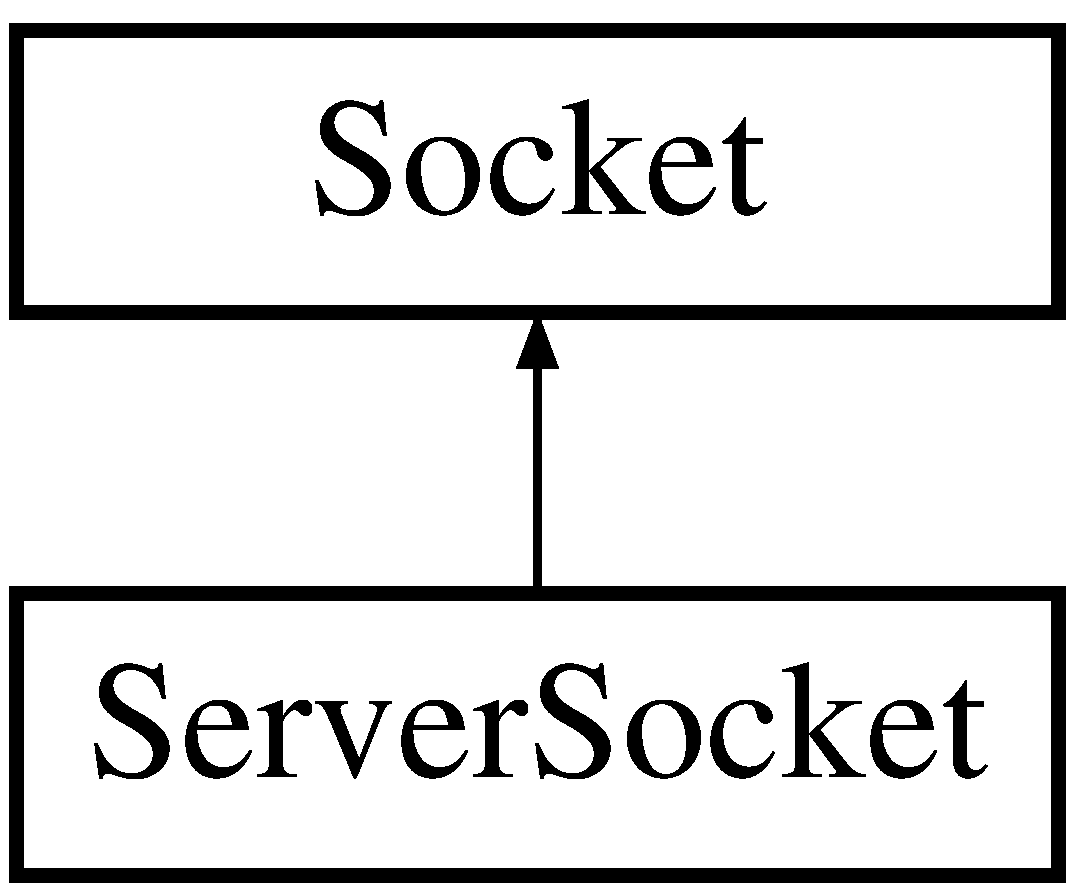
\includegraphics[height=2.000000cm]{classSocket}
\end{center}
\end{figure}
\subsection*{Public Member Functions}
\begin{DoxyCompactItemize}
\item 
\hyperlink{classSocket_a93c96fe7bea2fc834c88786629fa041e}{Socket} (int sd=-\/1)
\item 
\hyperlink{classSocket_aeac4eb6379a543d38ed88977d3b6630a}{$\sim$\+Socket} ()
\item 
\hyperlink{classSocket_a9016e6a1e5ae817f917449d5e3a7a380}{Socket} (const char $\ast$host, int port)
\item 
int \hyperlink{classSocket_abc97e53080c01a06cc8f5efea7c6cdf0}{connect} (const char $\ast$host, int port)
\item 
int \hyperlink{classSocket_aca3e5b9c5459a50bd8fb03d29ef9e48e}{send} (const char $\ast$msg, int len)
\item 
int \hyperlink{classSocket_a1830972b26797cde234054f81f0921de}{recv} (char $\ast$msg, int len)
\item 
void \hyperlink{classSocket_a75ee749264ccbcfc4dfbf5442e55dcb8}{close} ()
\item 
int \hyperlink{classSocket_a378077061dfb9c50e9db4b0d84ff2b03}{get\+Descriptor} ()
\item 
int \hyperlink{classSocket_a2b89fc6d75015cbf6abe93b2b9994ef4}{get\+Connected} ()
\end{DoxyCompactItemize}
\subsection*{Protected Member Functions}
\begin{DoxyCompactItemize}
\item 
void \hyperlink{classSocket_a23f2fbf5f8449277c7d140f32d12fca3}{create\+\_\+socket} ()
\end{DoxyCompactItemize}
\subsection*{Protected Attributes}
\begin{DoxyCompactItemize}
\item 
int \hyperlink{classSocket_a457f5e3f2429eb859f9e80f064073874}{descrip}
\item 
int \hyperlink{classSocket_af04394b9f1235562146aaa9291df70f8}{connected}
\end{DoxyCompactItemize}


\subsection{Detailed Description}
A class for socket communication 

\subsection{Constructor \& Destructor Documentation}
\hypertarget{classSocket_a93c96fe7bea2fc834c88786629fa041e}{}\index{Socket@{Socket}!Socket@{Socket}}
\index{Socket@{Socket}!Socket@{Socket}}
\subsubsection[{Socket(int sd=-\/1)}]{\setlength{\rightskip}{0pt plus 5cm}Socket\+::\+Socket (
\begin{DoxyParamCaption}
\item[{int}]{sd = {\ttfamily -\/1}}
\end{DoxyParamCaption}
)}\label{classSocket_a93c96fe7bea2fc834c88786629fa041e}

\begin{DoxyCode}
23                      \{
24   \textcolor{keywordflow}{if} (sd == -1) \{
25     \hyperlink{classSocket_a23f2fbf5f8449277c7d140f32d12fca3}{create\_socket}();
26   \} \textcolor{keywordflow}{else} \{
27     \hyperlink{classSocket_a457f5e3f2429eb859f9e80f064073874}{descrip} = sd;
28     \textcolor{keyword}{struct }sockaddr\_in ca; \textcolor{comment}{// socket address structure for the new client}
29     socklen\_t size = \textcolor{keyword}{sizeof}(\textcolor{keyword}{struct }sockaddr);
30     \textcolor{keywordflow}{if} (!::getpeername(sd, (\textcolor{keyword}{struct} sockaddr *)&ca, &size)) \{
31       \hyperlink{classSocket_af04394b9f1235562146aaa9291df70f8}{connected} = 1;
32     \} \textcolor{keywordflow}{else} \{
33       \hyperlink{classSocket_af04394b9f1235562146aaa9291df70f8}{connected} = 0;
34       \textcolor{keywordflow}{if} (errno != ENOTCONN)
35         cerr << \textcolor{stringliteral}{"Socket::Socket() getpeername "} << strerror(errno) << endl;
36     \}
37   \}
38 \}
\end{DoxyCode}
\hypertarget{classSocket_aeac4eb6379a543d38ed88977d3b6630a}{}\index{Socket@{Socket}!````~Socket@{$\sim$\+Socket}}
\index{````~Socket@{$\sim$\+Socket}!Socket@{Socket}}
\subsubsection[{$\sim$\+Socket()}]{\setlength{\rightskip}{0pt plus 5cm}Socket\+::$\sim$\+Socket (
\begin{DoxyParamCaption}
{}
\end{DoxyParamCaption}
)}\label{classSocket_aeac4eb6379a543d38ed88977d3b6630a}

\begin{DoxyCode}
45                 \{
46   \hyperlink{classSocket_a75ee749264ccbcfc4dfbf5442e55dcb8}{close}();
47 \}
\end{DoxyCode}
\hypertarget{classSocket_a9016e6a1e5ae817f917449d5e3a7a380}{}\index{Socket@{Socket}!Socket@{Socket}}
\index{Socket@{Socket}!Socket@{Socket}}
\subsubsection[{Socket(const char $\ast$host, int port)}]{\setlength{\rightskip}{0pt plus 5cm}Socket\+::\+Socket (
\begin{DoxyParamCaption}
\item[{const char $\ast$}]{host, }
\item[{int}]{port}
\end{DoxyParamCaption}
)}\label{classSocket_a9016e6a1e5ae817f917449d5e3a7a380}
initialize a socket and attempt to connect to a particular host and port 
\begin{DoxyParams}{Parameters}
{\em host} & Internet name for a computer, e.\+g., rns202-\/1.\+cs.\+stolaf.\+edu \\
\hline
{\em port} & T\+C\+P port for server socket on host \\
\hline
\end{DoxyParams}

\begin{DoxyCode}
40                                          \{
41   \hyperlink{classSocket_a23f2fbf5f8449277c7d140f32d12fca3}{create\_socket}();
42   \hyperlink{classSocket_abc97e53080c01a06cc8f5efea7c6cdf0}{connect}(host, port);
43 \}
\end{DoxyCode}


\subsection{Member Function Documentation}
\hypertarget{classSocket_a75ee749264ccbcfc4dfbf5442e55dcb8}{}\index{Socket@{Socket}!close@{close}}
\index{close@{close}!Socket@{Socket}}
\subsubsection[{close()}]{\setlength{\rightskip}{0pt plus 5cm}void Socket\+::close (
\begin{DoxyParamCaption}
{}
\end{DoxyParamCaption}
)}\label{classSocket_a75ee749264ccbcfc4dfbf5442e55dcb8}
Invalidate this socket for further use. If connected, first shut down communication. 
\begin{DoxyCode}
49                    \{
50   \textcolor{keywordflow}{if} (\hyperlink{classSocket_af04394b9f1235562146aaa9291df70f8}{connected} and ::shutdown(\hyperlink{classSocket_a457f5e3f2429eb859f9e80f064073874}{descrip}, SHUT\_RDWR) < 0)
51     cerr << \textcolor{stringliteral}{"Socket::close() shutdown "} << strerror(errno) << endl;
52   \hyperlink{classSocket_af04394b9f1235562146aaa9291df70f8}{connected} = 0;
53   \textcolor{keywordflow}{if} (::\hyperlink{classSocket_a75ee749264ccbcfc4dfbf5442e55dcb8}{close}(\hyperlink{classSocket_a457f5e3f2429eb859f9e80f064073874}{descrip}) < 0)
54     cerr << \textcolor{stringliteral}{"Socket::close() "} << strerror(errno) << endl;
55   \textcolor{comment}{// cout << "closed socket <" << descrip << ">" << endl; // DEBUG}
56 \}
\end{DoxyCode}
\hypertarget{classSocket_abc97e53080c01a06cc8f5efea7c6cdf0}{}\index{Socket@{Socket}!connect@{connect}}
\index{connect@{connect}!Socket@{Socket}}
\subsubsection[{connect(const char $\ast$host, int port)}]{\setlength{\rightskip}{0pt plus 5cm}int Socket\+::connect (
\begin{DoxyParamCaption}
\item[{const char $\ast$}]{host, }
\item[{int}]{port}
\end{DoxyParamCaption}
)}\label{classSocket_abc97e53080c01a06cc8f5efea7c6cdf0}
Connect this socket to a server \begin{DoxyPrecond}{Precondition}
State variable connected must be assigned before calling this method 
\end{DoxyPrecond}

\begin{DoxyParams}{Parameters}
{\em host} & Internet name for a computer, e.\+g., rns202-\/1.\+cs.\+stolaf.\+edu \\
\hline
{\em port} & T\+C\+P port for server socket on host \\
\hline
\end{DoxyParams}
\begin{DoxyReturn}{Returns}
1 on success, 0 on failure 
\end{DoxyReturn}

\begin{DoxyCode}
58                                               \{
59   \textcolor{keywordflow}{if} (\hyperlink{classSocket_af04394b9f1235562146aaa9291df70f8}{connected}) \{
60     cerr << \textcolor{stringliteral}{"Socket::connect() - already marked as connected, skipping"} << endl;
61     \textcolor{keywordflow}{return} 0;
62   \}
63   \textcolor{comment}{// connected == 0}
64 
65   \textcolor{keyword}{struct }hostent *hp;
66   \textcolor{keyword}{struct }sockaddr\_in sa;
67   \textcolor{keywordflow}{if} ((hp = gethostbyname(host)) == NULL) \{
68     cerr << \textcolor{stringliteral}{"Socket::connect() gethostbyname() "} << strerror(errno) << endl;
69     \textcolor{keywordflow}{return} 0;
70   \}
71   memset((\textcolor{keywordtype}{char} *)&sa, \textcolor{charliteral}{'\(\backslash\)0'}, \textcolor{keyword}{sizeof}(sa));
72   memcpy((\textcolor{keywordtype}{char} *)&sa.sin\_addr.s\_addr, hp->h\_addr, hp->h\_length);
73   sa.sin\_family = AF\_INET;
74   sa.sin\_port = htons(port);
75 
76   \textcolor{keywordflow}{if} (::\hyperlink{classSocket_abc97e53080c01a06cc8f5efea7c6cdf0}{connect}(\hyperlink{classSocket_a457f5e3f2429eb859f9e80f064073874}{descrip}, (\textcolor{keyword}{struct} sockaddr *)&sa, \textcolor{keyword}{sizeof}(sa)) < 0) \{
77     cerr << \textcolor{stringliteral}{"Socket::connect() "} << strerror(errno) << endl;
78     \textcolor{keywordflow}{if} (errno == EISCONN)
79       \hyperlink{classSocket_af04394b9f1235562146aaa9291df70f8}{connected} = 1;
80     \textcolor{keywordflow}{return} 0;
81   \}
82   \hyperlink{classSocket_af04394b9f1235562146aaa9291df70f8}{connected} = 1;
83   \textcolor{keywordflow}{return} 1;
84 \}
\end{DoxyCode}
\hypertarget{classSocket_a23f2fbf5f8449277c7d140f32d12fca3}{}\index{Socket@{Socket}!create\+\_\+socket@{create\+\_\+socket}}
\index{create\+\_\+socket@{create\+\_\+socket}!Socket@{Socket}}
\subsubsection[{create\+\_\+socket()}]{\setlength{\rightskip}{0pt plus 5cm}void Socket\+::create\+\_\+socket (
\begin{DoxyParamCaption}
{}
\end{DoxyParamCaption}
)\hspace{0.3cm}{\ttfamily [protected]}}\label{classSocket_a23f2fbf5f8449277c7d140f32d12fca3}
helper method for socket initialization \begin{DoxyParagraph}{State Changes}
Initialize descrip, and assign 0 to connected 
\end{DoxyParagraph}

\begin{DoxyCode}
17                            \{
18   \textcolor{keywordflow}{if} ((\hyperlink{classSocket_a457f5e3f2429eb859f9e80f064073874}{descrip} = socket(AF\_INET, SOCK\_STREAM, 0)) < 0)
19     cerr << \textcolor{stringliteral}{"Socket::Socket():"} << strerror(errno) << endl;
20   \hyperlink{classSocket_af04394b9f1235562146aaa9291df70f8}{connected} = 0;
21 \}
\end{DoxyCode}
\hypertarget{classSocket_a2b89fc6d75015cbf6abe93b2b9994ef4}{}\index{Socket@{Socket}!get\+Connected@{get\+Connected}}
\index{get\+Connected@{get\+Connected}!Socket@{Socket}}
\subsubsection[{get\+Connected()}]{\setlength{\rightskip}{0pt plus 5cm}int Socket\+::get\+Connected (
\begin{DoxyParamCaption}
{}
\end{DoxyParamCaption}
)\hspace{0.3cm}{\ttfamily [inline]}}\label{classSocket_a2b89fc6d75015cbf6abe93b2b9994ef4}
\begin{DoxyReturn}{Returns}
Value of state variable connected 
\end{DoxyReturn}

\begin{DoxyCode}
49 \{ \textcolor{keywordflow}{return} \hyperlink{classSocket_af04394b9f1235562146aaa9291df70f8}{connected}; \}
\end{DoxyCode}
\hypertarget{classSocket_a378077061dfb9c50e9db4b0d84ff2b03}{}\index{Socket@{Socket}!get\+Descriptor@{get\+Descriptor}}
\index{get\+Descriptor@{get\+Descriptor}!Socket@{Socket}}
\subsubsection[{get\+Descriptor()}]{\setlength{\rightskip}{0pt plus 5cm}int Socket\+::get\+Descriptor (
\begin{DoxyParamCaption}
{}
\end{DoxyParamCaption}
)\hspace{0.3cm}{\ttfamily [inline]}}\label{classSocket_a378077061dfb9c50e9db4b0d84ff2b03}
\begin{DoxyReturn}{Returns}
Value of state variable descrip 
\end{DoxyReturn}

\begin{DoxyCode}
46 \{ \textcolor{keywordflow}{return} \hyperlink{classSocket_a457f5e3f2429eb859f9e80f064073874}{descrip}; \}
\end{DoxyCode}
\hypertarget{classSocket_a1830972b26797cde234054f81f0921de}{}\index{Socket@{Socket}!recv@{recv}}
\index{recv@{recv}!Socket@{Socket}}
\subsubsection[{recv(char $\ast$msg, int len)}]{\setlength{\rightskip}{0pt plus 5cm}int Socket\+::recv (
\begin{DoxyParamCaption}
\item[{char $\ast$}]{msg, }
\item[{int}]{len}
\end{DoxyParamCaption}
)}\label{classSocket_a1830972b26797cde234054f81f0921de}
Receive a message on this socket 
\begin{DoxyParams}{Parameters}
{\em buff} & Array to receive message \\
\hline
{\em len} & Maximum number of characters to receive in buff \\
\hline
\end{DoxyParams}
\begin{DoxyReturn}{Returns}
Number of characters transmitted, or -\/1 on failure 
\end{DoxyReturn}

\begin{DoxyCode}
98                                     \{
99   \textcolor{keywordflow}{if} (!\hyperlink{classSocket_af04394b9f1235562146aaa9291df70f8}{connected}) \{
100     cerr << \textcolor{stringliteral}{"Attempt to recv() on a disconnected Socket"} << endl;
101     \textcolor{keywordflow}{return} -1;
102   \}
103 
104   \textcolor{keywordtype}{int} ret;
105   \textcolor{keywordflow}{if} ((ret = ::\hyperlink{classSocket_a1830972b26797cde234054f81f0921de}{recv}(\hyperlink{classSocket_a457f5e3f2429eb859f9e80f064073874}{descrip}, buff, len, 0)) < 0) \{
106     cerr << \textcolor{stringliteral}{"Socket::recv() "} << strerror(errno) << endl;
107     \textcolor{keywordflow}{return} -1;
108   \}
109   \textcolor{keywordflow}{return} ret;
110 \}
\end{DoxyCode}
\hypertarget{classSocket_aca3e5b9c5459a50bd8fb03d29ef9e48e}{}\index{Socket@{Socket}!send@{send}}
\index{send@{send}!Socket@{Socket}}
\subsubsection[{send(const char $\ast$msg, int len)}]{\setlength{\rightskip}{0pt plus 5cm}int Socket\+::send (
\begin{DoxyParamCaption}
\item[{const char $\ast$}]{msg, }
\item[{int}]{len}
\end{DoxyParamCaption}
)}\label{classSocket_aca3e5b9c5459a50bd8fb03d29ef9e48e}
Send a message on this socket 
\begin{DoxyParams}{Parameters}
{\em msg} & Message to be transmitted \\
\hline
{\em len} & Number of characters of msg to transmit \\
\hline
\end{DoxyParams}
\begin{DoxyReturn}{Returns}
Number of characters transmitted, or -\/1 on failure 
\end{DoxyReturn}

\begin{DoxyCode}
86                                          \{
87   \textcolor{keywordflow}{if} (!\hyperlink{classSocket_af04394b9f1235562146aaa9291df70f8}{connected}) \{
88     cerr << \textcolor{stringliteral}{"Attempt to send() on a disconnected Socket"} << endl;
89     \textcolor{keywordflow}{return} -1;
90   \}
91 
92   \textcolor{keywordtype}{int} ret;
93   \textcolor{keywordflow}{if} ((ret = ::\hyperlink{classSocket_aca3e5b9c5459a50bd8fb03d29ef9e48e}{send}(\hyperlink{classSocket_a457f5e3f2429eb859f9e80f064073874}{descrip}, msg, len, 0)) < 0)
94     cerr << \textcolor{stringliteral}{"Socket::send() "} << strerror(errno) << endl;
95   \textcolor{keywordflow}{return} ret;
96 \}
\end{DoxyCode}


\subsection{Member Data Documentation}
\hypertarget{classSocket_af04394b9f1235562146aaa9291df70f8}{}\index{Socket@{Socket}!connected@{connected}}
\index{connected@{connected}!Socket@{Socket}}
\subsubsection[{connected}]{\setlength{\rightskip}{0pt plus 5cm}int Socket\+::connected\hspace{0.3cm}{\ttfamily [protected]}}\label{classSocket_af04394b9f1235562146aaa9291df70f8}
non-\/zero if \hyperlink{classSocket_abc97e53080c01a06cc8f5efea7c6cdf0}{connect()} succeeded on this socket \hypertarget{classSocket_a457f5e3f2429eb859f9e80f064073874}{}\index{Socket@{Socket}!descrip@{descrip}}
\index{descrip@{descrip}!Socket@{Socket}}
\subsubsection[{descrip}]{\setlength{\rightskip}{0pt plus 5cm}int Socket\+::descrip\hspace{0.3cm}{\ttfamily [protected]}}\label{classSocket_a457f5e3f2429eb859f9e80f064073874}
socket descriptor, or -\/1 if failed to allocate socket 

The documentation for this class was generated from the following files\+:\begin{DoxyCompactItemize}
\item 
\hyperlink{Socket_8h}{Socket.\+h}\item 
\hyperlink{Socket_8cpp}{Socket.\+cpp}\end{DoxyCompactItemize}

\hypertarget{classWorker}{}\section{Worker Class Reference}
\label{classWorker}\index{Worker@{Worker}}


{\ttfamily \#include $<$Worker.\+h$>$}

Inheritance diagram for Worker\+:\begin{figure}[H]
\begin{center}
\leavevmode
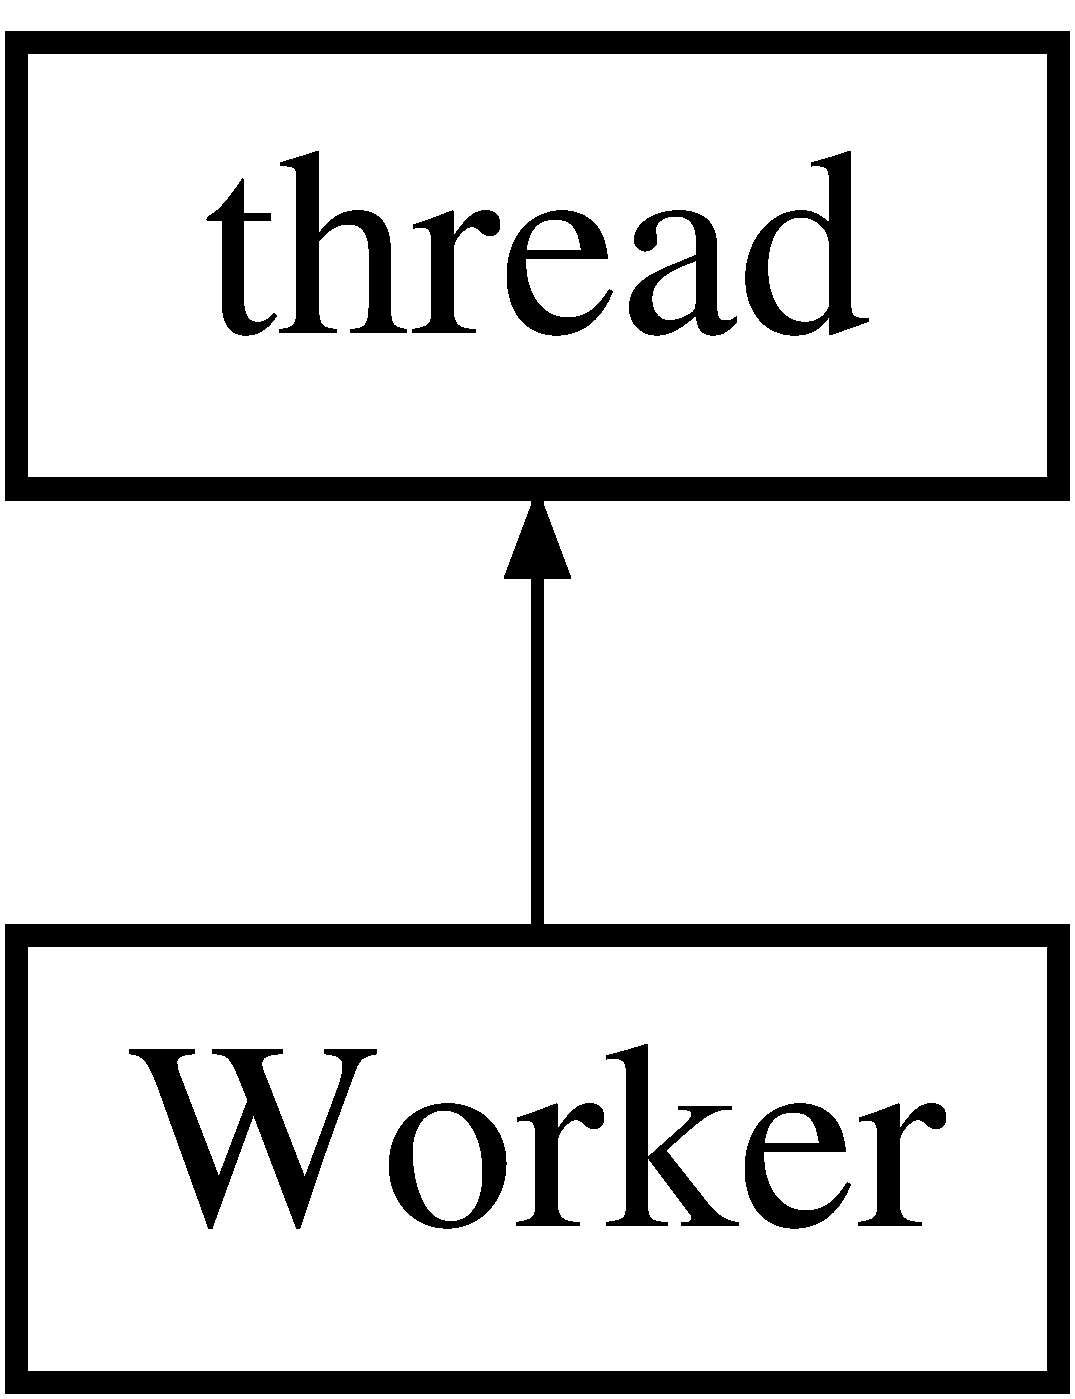
\includegraphics[height=2.000000cm]{classWorker}
\end{center}
\end{figure}
\subsection*{Public Member Functions}
\begin{DoxyCompactItemize}
\item 
\hyperlink{classWorker_a0a75e3ee66254224da70636e3ce40d8e}{Worker} (int i=-\/1, \hyperlink{classSocket}{Socket} $\ast$sp=0, const \hyperlink{structControlData}{Control\+Data} $\ast$cdp=0)
\item 
\hyperlink{classWorker_aa8e4543ef1e93fd9d884269ba30c5bfe}{$\sim$\+Worker} ()
\item 
\hyperlink{Worker_8h_ab3804a8a4369184ad46dadf8e54957b6}{Thread\+State} \hyperlink{classWorker_a2ababbc935eb10458640d2441f5e0c95}{get\+State} ()
\item 
int \hyperlink{classWorker_ac4629e67476bbb1daab8ed28545b8421}{get\+Id} ()
\end{DoxyCompactItemize}
\subsection*{Protected Member Functions}
\begin{DoxyCompactItemize}
\item 
void \hyperlink{classWorker_aeeb8e21ecb6687c34db1ad301028e41b}{do\+Work} (const \hyperlink{structControlData}{Control\+Data} $\ast$cdp)
\end{DoxyCompactItemize}
\subsection*{Protected Attributes}
\begin{DoxyCompactItemize}
\item 
int \hyperlink{classWorker_a50acebd9c077214060ff190bd54d351c}{id}
\item 
\hyperlink{classSocket}{Socket} $\ast$ \hyperlink{classWorker_a4562eb405aea20c7ac8a552e2075898f}{sockp}
\item 
\hyperlink{Worker_8h_ab3804a8a4369184ad46dadf8e54957b6}{Thread\+State} \hyperlink{classWorker_aeb90d4cd08a8a4759749c5388be8c78d}{state}
\end{DoxyCompactItemize}
\subsection*{Static Protected Attributes}
\begin{DoxyCompactItemize}
\item 
static int \hyperlink{classWorker_a2749db22d3591fe663b9a25e90a88e9d}{M\+A\+X\+B\+U\+F\+F} = 100
\end{DoxyCompactItemize}


\subsection{Detailed Description}
A class representing a thread that implements services for a client 

\subsection{Constructor \& Destructor Documentation}
\hypertarget{classWorker_a0a75e3ee66254224da70636e3ce40d8e}{}\index{Worker@{Worker}!Worker@{Worker}}
\index{Worker@{Worker}!Worker@{Worker}}
\subsubsection[{Worker(int i=-\/1, Socket $\ast$sp=0, const Control\+Data $\ast$cdp=0)}]{\setlength{\rightskip}{0pt plus 5cm}Worker\+::\+Worker (
\begin{DoxyParamCaption}
\item[{int}]{i = {\ttfamily -\/1}, }
\item[{{\bf Socket} $\ast$}]{sp = {\ttfamily 0}, }
\item[{const {\bf Control\+Data} $\ast$}]{cdp = {\ttfamily 0}}
\end{DoxyParamCaption}
)}\label{classWorker_a0a75e3ee66254224da70636e3ce40d8e}

\begin{DoxyParams}{Parameters}
{\em i} & I\+D number for this worker thread \\
\hline
{\em sp} & Pointer to socket for communicating with client \\
\hline
\end{DoxyParams}

\begin{DoxyCode}
11 : thread(&\hyperlink{classWorker_aeeb8e21ecb6687c34db1ad301028e41b}{Worker::doWork}, \textcolor{keyword}{this}, cdp), \hyperlink{classWorker_a50acebd9c077214060ff190bd54d351c}{id}(i), \hyperlink{classWorker_a4562eb405aea20c7ac8a552e2075898f}{sockp}(sp), 
      \hyperlink{classWorker_aeb90d4cd08a8a4759749c5388be8c78d}{state}(\hyperlink{Worker_8h_ab3804a8a4369184ad46dadf8e54957b6a1061be6c3fb88d32829cba6f6b2be304}{RUNNING}) \{\}
\end{DoxyCode}
\hypertarget{classWorker_aa8e4543ef1e93fd9d884269ba30c5bfe}{}\index{Worker@{Worker}!````~Worker@{$\sim$\+Worker}}
\index{````~Worker@{$\sim$\+Worker}!Worker@{Worker}}
\subsubsection[{$\sim$\+Worker()}]{\setlength{\rightskip}{0pt plus 5cm}Worker\+::$\sim$\+Worker (
\begin{DoxyParamCaption}
{}
\end{DoxyParamCaption}
)}\label{classWorker_aa8e4543ef1e93fd9d884269ba30c5bfe}

\begin{DoxyCode}
18                    \{
19     \textcolor{keyword}{delete} \hyperlink{classWorker_a4562eb405aea20c7ac8a552e2075898f}{sockp};
20     \hyperlink{classWorker_a4562eb405aea20c7ac8a552e2075898f}{sockp} = 0;
21   \}
\end{DoxyCode}


\subsection{Member Function Documentation}
\hypertarget{classWorker_aeeb8e21ecb6687c34db1ad301028e41b}{}\index{Worker@{Worker}!do\+Work@{do\+Work}}
\index{do\+Work@{do\+Work}!Worker@{Worker}}
\subsubsection[{do\+Work(const Control\+Data $\ast$cdp)}]{\setlength{\rightskip}{0pt plus 5cm}void Worker\+::do\+Work (
\begin{DoxyParamCaption}
\item[{const {\bf Control\+Data} $\ast$}]{cdp}
\end{DoxyParamCaption}
)\hspace{0.3cm}{\ttfamily [protected]}}\label{classWorker_aeeb8e21ecb6687c34db1ad301028e41b}

\begin{DoxyParams}{Parameters}
{\em cdp} & Points to shared data structure for controlling server \\
\hline
\end{DoxyParams}

\begin{DoxyCode}
23                                             \{
24   \textcolor{keywordtype}{char} buff[\hyperlink{classWorker_a2749db22d3591fe663b9a25e90a88e9d}{MAXBUFF}];  \textcolor{comment}{/* message buffer */}
25   \textcolor{keywordtype}{int} ret;  \textcolor{comment}{/* return value from a call */}
26 
27     cout << \textcolor{stringliteral}{"["} << \textcolor{keywordtype}{id} << \textcolor{stringliteral}{"] started"} << endl;
28   \textcolor{comment}{// cout << "[" << id << "] socket <" << sockp->getDescriptor() << ">" << endl; //DEBUG}
29 
30 
31   \textcolor{comment}{// send welcome message}
32     \textcolor{keywordflow}{if} (cdp->\hyperlink{structControlData_ac8fbf80345423cf5650ae64bfb10dc88}{contin}) 
33       strcpy(buff, \textcolor{stringliteral}{"ACK"});
34     \textcolor{keywordflow}{else}
35       strcpy(buff, \textcolor{stringliteral}{"DONE"});
36     \hyperlink{classWorker_a4562eb405aea20c7ac8a552e2075898f}{sockp}->\hyperlink{classSocket_aca3e5b9c5459a50bd8fb03d29ef9e48e}{send}(buff, strlen(buff));  
37 
38     \textcolor{keywordflow}{while} (strcmp(buff, \textcolor{stringliteral}{"DONE"}) != 0) \{
39       ret = \hyperlink{classWorker_a4562eb405aea20c7ac8a552e2075898f}{sockp}->\hyperlink{classSocket_a1830972b26797cde234054f81f0921de}{recv}(buff, \hyperlink{classWorker_a2749db22d3591fe663b9a25e90a88e9d}{MAXBUFF}-1);
40 
41     buff[ret] = \textcolor{charliteral}{'\(\backslash\)0'};  \textcolor{comment}{// add terminating nullbyte to received array of chars}
42     cout << \textcolor{stringliteral}{"["} << \textcolor{keywordtype}{id} << \textcolor{stringliteral}{"] Received message ("} << ret << \textcolor{stringliteral}{" chars):"} << endl 
43     << buff << endl;
44 
45     \textcolor{keywordflow}{if} (strcmp(buff, \textcolor{stringliteral}{"DONE"}) == 0 || !cdp->\hyperlink{structControlData_ac8fbf80345423cf5650ae64bfb10dc88}{contin}) \{
46       strcpy(buff, \textcolor{stringliteral}{"DONE"});
47       \hyperlink{classWorker_a4562eb405aea20c7ac8a552e2075898f}{sockp}->\hyperlink{classSocket_aca3e5b9c5459a50bd8fb03d29ef9e48e}{send}(buff, 4);
48       cout << \textcolor{stringliteral}{"["} << \textcolor{keywordtype}{id} << \textcolor{stringliteral}{"] sent termination message"} << endl;
49     \} \textcolor{keywordflow}{else} \textcolor{keywordflow}{if} (strncmp(buff, \textcolor{stringliteral}{"MSG "}, 4) == 0) \{
50       \hyperlink{classWorker_a4562eb405aea20c7ac8a552e2075898f}{sockp}->\hyperlink{classSocket_aca3e5b9c5459a50bd8fb03d29ef9e48e}{send}(\textcolor{stringliteral}{"ACK"}, 3);
51       cout << \textcolor{stringliteral}{"["} << \textcolor{keywordtype}{id} << \textcolor{stringliteral}{"] sent acknowledgment"} << endl;
52     \} \textcolor{keywordflow}{else} \textcolor{keywordflow}{if} (strncmp(buff, \textcolor{stringliteral}{"LINE1 "}, 6) == 0) \{
53 
54       ifstream f;
55       \textcolor{keywordtype}{char} fileName[20];
56       \textcolor{keywordflow}{for} (\textcolor{keywordtype}{int} n=6; buff[n] != \textcolor{charliteral}{'\(\backslash\)0'}; ++n)\{
57         fileName[n-6] = buff[n];
58       \}
59       f.open(fileName);
60       \textcolor{keywordflow}{if} (f.is\_open()) \{
61         \textcolor{keywordtype}{string} line;
62         getline(f, line);
63         cout << line << endl;
64         \textcolor{keywordtype}{int} n = line.length();
65         \hyperlink{classWorker_a4562eb405aea20c7ac8a552e2075898f}{sockp}->\hyperlink{classSocket_aca3e5b9c5459a50bd8fb03d29ef9e48e}{send}(line.c\_str(), n);
66         cout<<\textcolor{stringliteral}{"["}<<\textcolor{keywordtype}{id}<<\textcolor{stringliteral}{"] Returned line from file "}<<fileName<<endl;
67         f.close();
68       \}
69       \textcolor{keywordflow}{else} \{
70         \hyperlink{classWorker_a4562eb405aea20c7ac8a552e2075898f}{sockp}->\hyperlink{classSocket_aca3e5b9c5459a50bd8fb03d29ef9e48e}{send}(\textcolor{stringliteral}{"NACK"}, 4);
71         cout<<\textcolor{stringliteral}{"Worker: send negative NACK"}<<endl;
72       \}
73     \} \textcolor{keywordflow}{else} \{
74       \hyperlink{classWorker_a4562eb405aea20c7ac8a552e2075898f}{sockp}->\hyperlink{classSocket_aca3e5b9c5459a50bd8fb03d29ef9e48e}{send}(\textcolor{stringliteral}{"NACK"}, 4);
75       cout << \textcolor{stringliteral}{"["} << \textcolor{keywordtype}{id} << \textcolor{stringliteral}{"] sent negative acknowledgment"} << endl;
76     \}
77 
78   \}
79 
80   \textcolor{comment}{// receive END message from client}
81   \textcolor{keywordflow}{if} ((ret = \hyperlink{classWorker_a4562eb405aea20c7ac8a552e2075898f}{sockp}->\hyperlink{classSocket_a1830972b26797cde234054f81f0921de}{recv}(buff, \hyperlink{classWorker_a2749db22d3591fe663b9a25e90a88e9d}{MAXBUFF}-1)) != -1) \{
82     buff[ret] = \textcolor{charliteral}{'\(\backslash\)0'};
83     cout << \textcolor{stringliteral}{"["} << \textcolor{keywordtype}{id} << \textcolor{stringliteral}{"] Received "} << buff << \textcolor{stringliteral}{" from client"} << endl;
84   \}
85   \hyperlink{classWorker_aeb90d4cd08a8a4759749c5388be8c78d}{state} = \hyperlink{Worker_8h_ab3804a8a4369184ad46dadf8e54957b6a9c954bcf443428c80b0f107b3bc48749}{DONE};
86 \}
\end{DoxyCode}
\hypertarget{classWorker_ac4629e67476bbb1daab8ed28545b8421}{}\index{Worker@{Worker}!get\+Id@{get\+Id}}
\index{get\+Id@{get\+Id}!Worker@{Worker}}
\subsubsection[{get\+Id()}]{\setlength{\rightskip}{0pt plus 5cm}int Worker\+::get\+Id (
\begin{DoxyParamCaption}
{}
\end{DoxyParamCaption}
)\hspace{0.3cm}{\ttfamily [inline]}}\label{classWorker_ac4629e67476bbb1daab8ed28545b8421}

\begin{DoxyCode}
40 \{ \textcolor{keywordflow}{return} \hyperlink{classWorker_a50acebd9c077214060ff190bd54d351c}{id}; \}
\end{DoxyCode}
\hypertarget{classWorker_a2ababbc935eb10458640d2441f5e0c95}{}\index{Worker@{Worker}!get\+State@{get\+State}}
\index{get\+State@{get\+State}!Worker@{Worker}}
\subsubsection[{get\+State()}]{\setlength{\rightskip}{0pt plus 5cm}{\bf Thread\+State} Worker\+::get\+State (
\begin{DoxyParamCaption}
{}
\end{DoxyParamCaption}
)\hspace{0.3cm}{\ttfamily [inline]}}\label{classWorker_a2ababbc935eb10458640d2441f5e0c95}

\begin{DoxyCode}
39 \{ \textcolor{keywordflow}{return} \hyperlink{classWorker_aeb90d4cd08a8a4759749c5388be8c78d}{state}; \}
\end{DoxyCode}


\subsection{Member Data Documentation}
\hypertarget{classWorker_a50acebd9c077214060ff190bd54d351c}{}\index{Worker@{Worker}!id@{id}}
\index{id@{id}!Worker@{Worker}}
\subsubsection[{id}]{\setlength{\rightskip}{0pt plus 5cm}int Worker\+::id\hspace{0.3cm}{\ttfamily [protected]}}\label{classWorker_a50acebd9c077214060ff190bd54d351c}
unique identifier for this worker thread \hypertarget{classWorker_a2749db22d3591fe663b9a25e90a88e9d}{}\index{Worker@{Worker}!M\+A\+X\+B\+U\+F\+F@{M\+A\+X\+B\+U\+F\+F}}
\index{M\+A\+X\+B\+U\+F\+F@{M\+A\+X\+B\+U\+F\+F}!Worker@{Worker}}
\subsubsection[{M\+A\+X\+B\+U\+F\+F}]{\setlength{\rightskip}{0pt plus 5cm}int Worker\+::\+M\+A\+X\+B\+U\+F\+F = 100\hspace{0.3cm}{\ttfamily [static]}, {\ttfamily [protected]}}\label{classWorker_a2749db22d3591fe663b9a25e90a88e9d}
buffer size for socket communication \hypertarget{classWorker_a4562eb405aea20c7ac8a552e2075898f}{}\index{Worker@{Worker}!sockp@{sockp}}
\index{sockp@{sockp}!Worker@{Worker}}
\subsubsection[{sockp}]{\setlength{\rightskip}{0pt plus 5cm}{\bf Socket}$\ast$ Worker\+::sockp\hspace{0.3cm}{\ttfamily [protected]}}\label{classWorker_a4562eb405aea20c7ac8a552e2075898f}
socket for communicating with client \hypertarget{classWorker_aeb90d4cd08a8a4759749c5388be8c78d}{}\index{Worker@{Worker}!state@{state}}
\index{state@{state}!Worker@{Worker}}
\subsubsection[{state}]{\setlength{\rightskip}{0pt plus 5cm}{\bf Thread\+State} Worker\+::state\hspace{0.3cm}{\ttfamily [protected]}}\label{classWorker_aeb90d4cd08a8a4759749c5388be8c78d}
current status of this worker thread 

The documentation for this class was generated from the following files\+:\begin{DoxyCompactItemize}
\item 
\hyperlink{Worker_8h}{Worker.\+h}\item 
\hyperlink{Worker_8cpp}{Worker.\+cpp}\end{DoxyCompactItemize}

\chapter{File Documentation}
\hypertarget{client_8cpp}{}\section{client.\+cpp File Reference}
\label{client_8cpp}\index{client.\+cpp@{client.\+cpp}}
{\ttfamily \#include $<$iostream$>$}\\*
{\ttfamily \#include $<$cstring$>$}\\*
{\ttfamily \#include \char`\"{}Socket.\+h\char`\"{}}\\*
\subsection*{Macros}
\begin{DoxyCompactItemize}
\item 
\#define \hyperlink{client_8cpp_a0c8dad16ba61ded55d3f302a616c0ced}{M\+A\+X\+B\+U\+F\+F}~100
\end{DoxyCompactItemize}
\subsection*{Functions}
\begin{DoxyCompactItemize}
\item 
int \hyperlink{client_8cpp_a3c04138a5bfe5d72780bb7e82a18e627}{main} (int argc, char $\ast$$\ast$argv)
\end{DoxyCompactItemize}


\subsection{Macro Definition Documentation}
\hypertarget{client_8cpp_a0c8dad16ba61ded55d3f302a616c0ced}{}\index{client.\+cpp@{client.\+cpp}!M\+A\+X\+B\+U\+F\+F@{M\+A\+X\+B\+U\+F\+F}}
\index{M\+A\+X\+B\+U\+F\+F@{M\+A\+X\+B\+U\+F\+F}!client.\+cpp@{client.\+cpp}}
\subsubsection[{M\+A\+X\+B\+U\+F\+F}]{\setlength{\rightskip}{0pt plus 5cm}\#define M\+A\+X\+B\+U\+F\+F~100}\label{client_8cpp_a0c8dad16ba61ded55d3f302a616c0ced}


\subsection{Function Documentation}
\hypertarget{client_8cpp_a3c04138a5bfe5d72780bb7e82a18e627}{}\index{client.\+cpp@{client.\+cpp}!main@{main}}
\index{main@{main}!client.\+cpp@{client.\+cpp}}
\subsubsection[{main(int argc, char $\ast$$\ast$argv)}]{\setlength{\rightskip}{0pt plus 5cm}int main (
\begin{DoxyParamCaption}
\item[{int}]{argc, }
\item[{char $\ast$$\ast$}]{argv}
\end{DoxyParamCaption}
)}\label{client_8cpp_a3c04138a5bfe5d72780bb7e82a18e627}

\begin{DoxyCode}
15                                 \{
16   \textcolor{keywordtype}{char} *prog = argv[0];
17   \textcolor{keywordtype}{char} *host;
18   \textcolor{keywordtype}{int} port;
19   \textcolor{keywordtype}{int} ret; \textcolor{comment}{/* return value from a call */}
20 
21   \textcolor{keywordflow}{if} (argc < 3) \{
22     cout << \textcolor{stringliteral}{"Usage:  "} << prog << \textcolor{stringliteral}{" host port"} << endl;
23     \textcolor{keywordflow}{return} 1;
24   \}
25   host = argv[1];
26   port = atoi(argv[2]);
27 
28   \hyperlink{classSocket}{Socket} sock(host, port);
29   \textcolor{keywordflow}{if} (sock.getConnected())
30     cout << \textcolor{stringliteral}{"Connected."} << endl;
31   \textcolor{keywordflow}{else} \{
32     cout << \textcolor{stringliteral}{"Could not connect, aborting"} << endl;
33     \textcolor{keywordflow}{return} 1;
34   \}
35 
36   \textcolor{keywordtype}{char} buff[\hyperlink{client_8cpp_a0c8dad16ba61ded55d3f302a616c0ced}{MAXBUFF}];       \textcolor{comment}{/* message buffer */}
37   \textcolor{keywordtype}{char} buff2[\hyperlink{client_8cpp_a0c8dad16ba61ded55d3f302a616c0ced}{MAXBUFF} + 10]; \textcolor{comment}{/* message buffer with prepended message type */}
38 
39   \textcolor{keywordflow}{if} ((ret = sock.recv(buff, \hyperlink{client_8cpp_a0c8dad16ba61ded55d3f302a616c0ced}{MAXBUFF} - 1)) < 0) \{
40     cout << \textcolor{stringliteral}{"Could not receive welcome message from server, aborting"} << endl;
41     \textcolor{keywordflow}{return} 1;
42   \}
43   buff[ret] = \textcolor{charliteral}{'\(\backslash\)0'};
44   \textcolor{keywordflow}{if} (strcmp(buff, \textcolor{stringliteral}{"NACK"}) == 0) \{
45     cout << \textcolor{stringliteral}{"Server rejected new connection, aborting"} << endl;
46     \textcolor{keywordflow}{return} 1;
47   \}
48   \textcolor{comment}{// assert:  welcome message received and connection to server completed}
49 
50   \textcolor{keywordflow}{while} (strcmp(buff, \textcolor{stringliteral}{"DONE"}) != 0) \{
51     cout << \textcolor{stringliteral}{"Enter a one-line message to send (max "} << \hyperlink{client_8cpp_a0c8dad16ba61ded55d3f302a616c0ced}{MAXBUFF} - 1
52          << \textcolor{stringliteral}{" chars), or DONE to quit"} << endl;
53     \textcolor{keywordflow}{if} (!cin.getline(buff, \hyperlink{client_8cpp_a0c8dad16ba61ded55d3f302a616c0ced}{MAXBUFF})) \{
54       cout << \textcolor{stringliteral}{"Error or end of input -- aborting"} << endl;
55       \textcolor{keywordflow}{return} 1;
56     \}
57     \textcolor{keywordflow}{if} (strcmp(buff, \textcolor{stringliteral}{"DONE"}) == 0)
58       strcpy(buff2, buff);
59     \textcolor{keywordflow}{else} \{
60       strcpy(buff2, \textcolor{stringliteral}{"MSG "});
61       strcat(buff2, buff);
62     \}
63     \textcolor{keywordflow}{if} ((ret = sock.send(buff2, strlen(buff2))) < 0)
64       \textcolor{keywordflow}{return} 1;
65     cout << ret << \textcolor{stringliteral}{" characters sent"} << endl;
66 
67     \textcolor{keywordflow}{if} ((ret = sock.recv(buff, \hyperlink{client_8cpp_a0c8dad16ba61ded55d3f302a616c0ced}{MAXBUFF} - 1)) < 0)
68       \textcolor{keywordflow}{return} 1;
69     \textcolor{keywordflow}{else} \{
70       buff[ret] = \textcolor{charliteral}{'\(\backslash\)0'};
71       cout << \textcolor{stringliteral}{"acknowledged "} << buff << endl;
72     \}
73   \}
74 
75   cout << \textcolor{stringliteral}{"Termination message received"} << endl;
76   sock.send(\textcolor{stringliteral}{"END"}, 3);
77   \textcolor{keywordflow}{return} 0;
78 \}
\end{DoxyCode}

\hypertarget{PiClasses_8cpp}{}\section{Pi\+Classes.\+cpp File Reference}
\label{PiClasses_8cpp}\index{Pi\+Classes.\+cpp@{Pi\+Classes.\+cpp}}
{\ttfamily \#include $<$iostream$>$}\\*
{\ttfamily \#include \char`\"{}Pi\+Classes.\+h\char`\"{}}\\*

\hypertarget{PiClasses_8h}{}\section{Pi\+Classes.\+h File Reference}
\label{PiClasses_8h}\index{Pi\+Classes.\+h@{Pi\+Classes.\+h}}
{\ttfamily \#include $<$sstream$>$}\\*
{\ttfamily \#include $<$fstream$>$}\\*
{\ttfamily \#include $<$string$>$}\\*
{\ttfamily \#include $<$unistd.\+h$>$}\\*
{\ttfamily \#include $<$cstring$>$}\\*
{\ttfamily \#include $<$sys/time.\+h$>$}\\*
\subsection*{Classes}
\begin{DoxyCompactItemize}
\item 
class \hyperlink{classMachine}{Machine}
\item 
class \hyperlink{classMovementData}{Movement\+Data}
\end{DoxyCompactItemize}

\hypertarget{pro4_8cpp}{}\section{pro4.\+cpp File Reference}
\label{pro4_8cpp}\index{pro4.\+cpp@{pro4.\+cpp}}
{\ttfamily \#include $<$iostream$>$}\\*
{\ttfamily \#include $<$sstream$>$}\\*
{\ttfamily \#include $<$fstream$>$}\\*
{\ttfamily \#include $<$string$>$}\\*
{\ttfamily \#include $<$unistd.\+h$>$}\\*
{\ttfamily \#include $<$cstring$>$}\\*
{\ttfamily \#include $<$thread$>$}\\*
{\ttfamily \#include $<$sys/time.\+h$>$}\\*
{\ttfamily \#include \char`\"{}Pi\+Classes.\+h\char`\"{}}\\*
{\ttfamily \#include \char`\"{}Worker.\+h\char`\"{}}\\*
\subsection*{Macros}
\begin{DoxyCompactItemize}
\item 
\#define \hyperlink{pro4_8cpp_a150aa807a94411b028b908cde770e0fe}{M\+A\+X\+W\+O\+R\+K\+E\+R\+S}~10
\end{DoxyCompactItemize}
\subsection*{Functions}
\begin{DoxyCompactItemize}
\item 
void \hyperlink{pro4_8cpp_a54a4c7d17db93a6dda7546a073e61b72}{do\+Control} (\hyperlink{structControlData}{Control\+Data} $\ast$cdp, int port)
\item 
void \hyperlink{pro4_8cpp_a91f84e64446f72dddee9e3eed8f44c01}{Sensor\+Program} (void)
\item 
int \hyperlink{pro4_8cpp_ae66f6b31b5ad750f1fe042a706a4e3d4}{main} ()
\end{DoxyCompactItemize}


\subsection{Macro Definition Documentation}
\hypertarget{pro4_8cpp_a150aa807a94411b028b908cde770e0fe}{}\index{pro4.\+cpp@{pro4.\+cpp}!M\+A\+X\+W\+O\+R\+K\+E\+R\+S@{M\+A\+X\+W\+O\+R\+K\+E\+R\+S}}
\index{M\+A\+X\+W\+O\+R\+K\+E\+R\+S@{M\+A\+X\+W\+O\+R\+K\+E\+R\+S}!pro4.\+cpp@{pro4.\+cpp}}
\subsubsection[{M\+A\+X\+W\+O\+R\+K\+E\+R\+S}]{\setlength{\rightskip}{0pt plus 5cm}\#define M\+A\+X\+W\+O\+R\+K\+E\+R\+S~10}\label{pro4_8cpp_a150aa807a94411b028b908cde770e0fe}


\subsection{Function Documentation}
\hypertarget{pro4_8cpp_a54a4c7d17db93a6dda7546a073e61b72}{}\index{pro4.\+cpp@{pro4.\+cpp}!do\+Control@{do\+Control}}
\index{do\+Control@{do\+Control}!pro4.\+cpp@{pro4.\+cpp}}
\subsubsection[{do\+Control(\+Control\+Data $\ast$cdp, int port)}]{\setlength{\rightskip}{0pt plus 5cm}void do\+Control (
\begin{DoxyParamCaption}
\item[{{\bf Control\+Data} $\ast$}]{cdp, }
\item[{int}]{port}
\end{DoxyParamCaption}
)}\label{pro4_8cpp_a54a4c7d17db93a6dda7546a073e61b72}
code for control thread 
\begin{DoxyParams}{Parameters}
{\em cdp} & points to smakhared data structure for controlling server \\
\hline
\end{DoxyParams}

\begin{DoxyCode}
21                                            \{
22   \textcolor{keyword}{const} \textcolor{keywordtype}{int} maxbuff = 100;
23   \textcolor{keywordtype}{char} buff[maxbuff];
24   \textcolor{keywordflow}{while} (cin.getline(buff, maxbuff - 1)) \{
25     \textcolor{keywordflow}{if} (strcmp(buff, \textcolor{stringliteral}{"EXIT"}) == 0)
26       \textcolor{keywordflow}{break};
27     \textcolor{keywordflow}{else}
28       cerr << \textcolor{stringliteral}{"[control thread] unrecognized command: "} << buff << endl;
29   \}
30 
31   \textcolor{comment}{// assert:  buff == "EXIT"}
32   cout << \textcolor{stringliteral}{"[control thread] EXIT encountered"} << endl;
33   cdp->\hyperlink{structControlData_ac8fbf80345423cf5650ae64bfb10dc88}{contin} = 0;
34 
35   \textcolor{comment}{// initialize as a Client, to unblock [main] accept()}
36   \hyperlink{classSocket}{Socket} sock(\textcolor{stringliteral}{"localhost"}, port);
37   sock.recv(buff, maxbuff - 1); \textcolor{comment}{// welcome message}
38 
39   \textcolor{comment}{//}
40   sock.send(\textcolor{stringliteral}{"DONE"}, 4);
41 \}
\end{DoxyCode}
\hypertarget{pro4_8cpp_ae66f6b31b5ad750f1fe042a706a4e3d4}{}\index{pro4.\+cpp@{pro4.\+cpp}!main@{main}}
\index{main@{main}!pro4.\+cpp@{pro4.\+cpp}}
\subsubsection[{main()}]{\setlength{\rightskip}{0pt plus 5cm}int main (
\begin{DoxyParamCaption}
{}
\end{DoxyParamCaption}
)}\label{pro4_8cpp_ae66f6b31b5ad750f1fe042a706a4e3d4}

\begin{DoxyCode}
95           \{             \textcolor{comment}{//main program}
96 
97   ifstream idStream;                \textcolor{comment}{//open the idfile to get macine Id and port number for connection}
98   \textcolor{keywordtype}{int} port;
99   \textcolor{keywordtype}{char} MachineId[13];
100   idStream.open(\textcolor{stringliteral}{"idfile.dat"});
101   \textcolor{keywordflow}{if} (idStream.good())\{
102       idStream>>MachineId;
103       cout<<\textcolor{stringliteral}{"Machine Id:"}<<MachineId<<endl;
104       idStream>>port;
105       idStream.close();
106   \}
107   \textcolor{keywordflow}{else}\{
108       cout<<\textcolor{stringliteral}{"idfile.dat not found"}<<endl;
109       \textcolor{keywordflow}{return} 1;
110   \}
111   \textcolor{comment}{//cout<<"Connection to socket "<<port<<endl;}
112 
113   \hyperlink{classServerSocket}{ServerSocket} ssock(port);
114   \textcolor{keywordflow}{if} (ssock.getBound())
115     cout << \textcolor{stringliteral}{"[main] port "} << port << \textcolor{stringliteral}{" bound to server socket"} << endl;
116   \textcolor{keywordflow}{else} \{
117     cout << \textcolor{stringliteral}{"[main] could not bind port "} << port
118          << \textcolor{stringliteral}{" to server socket, aborting"} << endl;
119     \textcolor{keywordflow}{return} 1;
120   \}
121   \textcolor{comment}{// server socket ssock is now set up}
122 
123   \textcolor{comment}{/* Define shared data structure for controlling server */}
124   \hyperlink{structControlData}{ControlData} controlData;
125 
126   \textcolor{comment}{/* Create a thread for handling control input */}
127   thread controlThread(\hyperlink{pro4_8cpp_a54a4c7d17db93a6dda7546a073e61b72}{doControl}, &controlData, port);
128   thread Thread2(\hyperlink{pro4_8cpp_a91f84e64446f72dddee9e3eed8f44c01}{SensorProgram});
129 
130   \textcolor{comment}{/* main loop: */}
131   \hyperlink{classSocket}{Socket} *csockp; \textcolor{comment}{// to hold new client socket}
132   \hyperlink{classWorker}{Worker} *workers[\hyperlink{pro4_8cpp_a150aa807a94411b028b908cde770e0fe}{MAXWORKERS}];
133   \textcolor{keywordflow}{for} (\textcolor{keywordtype}{int} i = 0; i < \hyperlink{pro4_8cpp_a150aa807a94411b028b908cde770e0fe}{MAXWORKERS}; i++)
134     workers[i] = 0;
135   \textcolor{keywordtype}{int} workerCount = 0;
136   \textcolor{keywordflow}{while} (controlData.\hyperlink{structControlData_ac8fbf80345423cf5650ae64bfb10dc88}{contin}) \{
137     csockp = ssock.accept();
138 
139     \textcolor{keywordtype}{int} indx = 0; \textcolor{comment}{// loop control for finding unused element in workers[]}
140     \textcolor{keywordflow}{while} (indx < MAXWORKERS) \{
141       \textcolor{keywordflow}{if} (workers[indx] != 0 &&
142           workers[indx]->getState() == \hyperlink{Worker_8h_ab3804a8a4369184ad46dadf8e54957b6a9c954bcf443428c80b0f107b3bc48749}{ThreadState::DONE}) \{
143         cout << \textcolor{stringliteral}{"[main] joining on ["} << workers[indx]->\hyperlink{classWorker_ac4629e67476bbb1daab8ed28545b8421}{getId}() << \textcolor{stringliteral}{"]"} << endl;
144         workers[indx]->join();
145         cout << \textcolor{stringliteral}{"[main] join on ["} << workers[indx]->\hyperlink{classWorker_ac4629e67476bbb1daab8ed28545b8421}{getId}() << \textcolor{stringliteral}{"] accomplished"}
146              << endl;
147         \textcolor{keyword}{delete} workers[indx];
148         workers[indx] = 0;
149       \}
150       \textcolor{keywordflow}{if} (workers[indx] == 0)
151         \textcolor{keywordflow}{break};
152       indx++;
153     \}
154     \textcolor{keywordflow}{if} (indx == MAXWORKERS) \{
155       cout << \textcolor{stringliteral}{"[main] workers[] overfull, rejecting a new client"} << endl;
156       csockp->\hyperlink{classSocket_aca3e5b9c5459a50bd8fb03d29ef9e48e}{send}(\textcolor{stringliteral}{"SVBG"}, 4); \textcolor{comment}{// server is busy, send error code back to client}
157       cout << \textcolor{stringliteral}{"SVBG sent"} << endl;
158       \textcolor{keywordflow}{continue};
159     \}
160 
161     workers[indx] =
162         \textcolor{keyword}{new} \hyperlink{classWorker}{Worker}(workerCount++, csockp, &controlData, MachineId);      \textcolor{comment}{//creating a new worker
       class (thread) after a connection request is recieved}
163   \}
164 
165   \textcolor{keywordflow}{for} (\textcolor{keywordtype}{int} i = 0; i < \hyperlink{pro4_8cpp_a150aa807a94411b028b908cde770e0fe}{MAXWORKERS}; i++)
166     \textcolor{keywordflow}{if} (workers[i]) \{
167       cout << \textcolor{stringliteral}{"[main] joining on ["} << workers[i]->\hyperlink{classWorker_ac4629e67476bbb1daab8ed28545b8421}{getId}() << \textcolor{stringliteral}{"]"} << endl;
168       workers[i]->join();
169       cout << \textcolor{stringliteral}{"[main] join on ["} << workers[i]->\hyperlink{classWorker_ac4629e67476bbb1daab8ed28545b8421}{getId}() << \textcolor{stringliteral}{"] accomplished"}
170            << endl;
171       \textcolor{keyword}{delete} workers[i];
172       workers[i] = 0;
173     \}
174 
175   controlThread.join();
176   Thread2.join();
177   cout << \textcolor{stringliteral}{"[main] control thread join accomplished"} << endl;
178 
179   \textcolor{keywordflow}{return} 0;
180 \}
\end{DoxyCode}
\hypertarget{pro4_8cpp_a91f84e64446f72dddee9e3eed8f44c01}{}\index{pro4.\+cpp@{pro4.\+cpp}!Sensor\+Program@{Sensor\+Program}}
\index{Sensor\+Program@{Sensor\+Program}!pro4.\+cpp@{pro4.\+cpp}}
\subsubsection[{Sensor\+Program(void)}]{\setlength{\rightskip}{0pt plus 5cm}void Sensor\+Program (
\begin{DoxyParamCaption}
\item[{void}]{}
\end{DoxyParamCaption}
)}\label{pro4_8cpp_a91f84e64446f72dddee9e3eed8f44c01}
code for thread tht deals with getting sensor data from serial port, analyzing it, deciding the status and timer of machine and updating the status file 
\begin{DoxyCode}
44                          \{
45 
46 \textcolor{comment}{//open the file contating address to serial port to get real time sensor data}
47   ifstream idStream;     
48   idStream.open(\textcolor{stringliteral}{"idfile.dat"});
49   \textcolor{keywordtype}{string} serialObt;
50   \textcolor{keywordflow}{for} (\textcolor{keywordtype}{int} i = 1; i <= 3; i++)    \textcolor{comment}{//go to the third line to get the address to serial port}
51       getline(idStream, serialObt);
52   \textcolor{keywordtype}{char} serialAd[13];
53   strcpy(serialAd, serialObt.c\_str());
54   serialAd[12]=\textcolor{charliteral}{'\(\backslash\)0'};
55   cout<<\textcolor{stringliteral}{"Serial Address:--"} <<serialAd<<\textcolor{stringliteral}{"--"}<<endl;
56   idStream.close();
57 
58   \hyperlink{classMovementData}{MovementData} M1;     \textcolor{comment}{//make a Machine class that represents this specific machine}
59   \textcolor{keywordtype}{string} data;
60   ifstream filestream;
61   filestream.open(serialAd);         \textcolor{comment}{//open the virtual serial port to get the vibration data}
62   \textcolor{keywordflow}{if} (filestream.good()) \{
63     M1.\hyperlink{classMachine_aae30fc95cd4f4089b79bcd680cf774eb}{setResponse}(1);                \textcolor{comment}{//set response as 1 or 0 if the arduino is found/not found}
64     \textcolor{keywordflow}{while} (1) \{
65       M1.\hyperlink{classMachine_aa2691fd518ccf5bf91f641d168c6e67d}{setFileAsNOTUSED}();          \textcolor{comment}{//set inital status as machine not used}
66 
67       \textcolor{keywordflow}{if} (M1.\hyperlink{classMovementData_a0460eb813078fc9e9eef646bb495a8a3}{contVibCheck}(filestream)) \{           \textcolor{comment}{//check for continuous vibration of machine}
68         cout << \textcolor{stringliteral}{"Machine Started"} << endl;
69         \textcolor{keywordtype}{double} startTime = M1.\hyperlink{classMachine_a2fb11e330fa5e2b6a7134ee55ac7ef43}{getCurrentTime}();      \textcolor{comment}{//record the start time}
70         \textcolor{keywordtype}{double} duration = 0;
71         \textcolor{keywordtype}{int} counter = 1;
72         \textcolor{keywordflow}{while} (duration < M1.\hyperlink{classMovementData_abd2ebde61b24ecee8634bc0ad5a9d79c}{CYCLEDURATION}) \{            \textcolor{comment}{//run the loop until cycle ends}
73           duration = M1.\hyperlink{classMachine_a2fb11e330fa5e2b6a7134ee55ac7ef43}{getCurrentTime}() - startTime;    \textcolor{comment}{//caculate timer}
74           counter++;                         \textcolor{comment}{//counter facilitates to create delay while accessing file to
       avoid race conditions}
75           \textcolor{keywordflow}{if} (counter % 10000000 == 0) \{                         
76             \textcolor{keywordtype}{double} timeleft = (M1.\hyperlink{classMovementData_abd2ebde61b24ecee8634bc0ad5a9d79c}{CYCLEDURATION} - duration) / 60;     \textcolor{comment}{//update status and
       timer in file}
77             M1.\hyperlink{classMachine_a2596d7951c310917a62a2be50ff62b5a}{setFileAsUSE}((\textcolor{keywordtype}{int})timeleft + 1);                    
78             counter = 0;
79           \}
80         \}
81         cout << \textcolor{stringliteral}{"Machine Stopped"} << endl;              \textcolor{comment}{//change status after timer is over and machine is
       unused again}
82         M1.\hyperlink{classMachine_aa2691fd518ccf5bf91f641d168c6e67d}{setFileAsNOTUSED}();
83       \}
84     \}
85   \}
86 
87   \textcolor{keywordflow}{else} \{
88     M1.\hyperlink{classMachine_aae30fc95cd4f4089b79bcd680cf774eb}{setResponse}(0);                 \textcolor{comment}{//set response as false is sensor isn' connected or isn't
       respondng}
89     M1.\hyperlink{classMachine_aa9451bf11291573e776f72305b41646f}{setAsNoSensor}();
90     cout<<\textcolor{stringliteral}{"Type EXIT to safely close the socket and exit."}<<endl;
91   \}
92 \}
\end{DoxyCode}

\hypertarget{Socket_8cpp}{}\section{Socket.\+cpp File Reference}
\label{Socket_8cpp}\index{Socket.\+cpp@{Socket.\+cpp}}
{\ttfamily \#include $<$iostream$>$}\\*
{\ttfamily \#include $<$cstdlib$>$}\\*
{\ttfamily \#include $<$cerrno$>$}\\*
{\ttfamily \#include $<$cstring$>$}\\*
{\ttfamily \#include $<$sys/types.\+h$>$}\\*
{\ttfamily \#include $<$sys/socket.\+h$>$}\\*
{\ttfamily \#include $<$netdb.\+h$>$}\\*
{\ttfamily \#include $<$netinet/in.\+h$>$}\\*
{\ttfamily \#include $<$unistd.\+h$>$}\\*
{\ttfamily \#include \char`\"{}Socket.\+h\char`\"{}}\\*

\hypertarget{Socket_8h}{}\section{Socket.\+h File Reference}
\label{Socket_8h}\index{Socket.\+h@{Socket.\+h}}
\subsection*{Classes}
\begin{DoxyCompactItemize}
\item 
class \hyperlink{classSocket}{Socket}
\item 
class \hyperlink{classServerSocket}{Server\+Socket}
\end{DoxyCompactItemize}

\hypertarget{Worker_8cpp}{}\section{Worker.\+cpp File Reference}
\label{Worker_8cpp}\index{Worker.\+cpp@{Worker.\+cpp}}
{\ttfamily \#include $<$iostream$>$}\\*
{\ttfamily \#include $<$fstream$>$}\\*
{\ttfamily \#include $<$cstring$>$}\\*
{\ttfamily \#include $<$thread$>$}\\*
{\ttfamily \#include \char`\"{}Worker.\+h\char`\"{}}\\*
\subsection*{Macros}
\begin{DoxyCompactItemize}
\item 
\#define \hyperlink{Worker_8cpp_a0c8dad16ba61ded55d3f302a616c0ced}{M\+A\+X\+B\+U\+F\+F}~13
\end{DoxyCompactItemize}


\subsection{Macro Definition Documentation}
\hypertarget{Worker_8cpp_a0c8dad16ba61ded55d3f302a616c0ced}{}\index{Worker.\+cpp@{Worker.\+cpp}!M\+A\+X\+B\+U\+F\+F@{M\+A\+X\+B\+U\+F\+F}}
\index{M\+A\+X\+B\+U\+F\+F@{M\+A\+X\+B\+U\+F\+F}!Worker.\+cpp@{Worker.\+cpp}}
\subsubsection[{M\+A\+X\+B\+U\+F\+F}]{\setlength{\rightskip}{0pt plus 5cm}\#define M\+A\+X\+B\+U\+F\+F~13}\label{Worker_8cpp_a0c8dad16ba61ded55d3f302a616c0ced}

\hypertarget{Worker_8h}{}\section{Worker.\+h File Reference}
\label{Worker_8h}\index{Worker.\+h@{Worker.\+h}}
{\ttfamily \#include $<$thread$>$}\\*
{\ttfamily \#include $<$atomic$>$}\\*
{\ttfamily \#include \char`\"{}Socket.\+h\char`\"{}}\\*
\subsection*{Classes}
\begin{DoxyCompactItemize}
\item 
struct \hyperlink{structControlData}{Control\+Data}
\item 
class \hyperlink{classWorker}{Worker}
\end{DoxyCompactItemize}
\subsection*{Enumerations}
\begin{DoxyCompactItemize}
\item 
enum \hyperlink{Worker_8h_ab3804a8a4369184ad46dadf8e54957b6}{Thread\+State} \{ \hyperlink{Worker_8h_ab3804a8a4369184ad46dadf8e54957b6a1061be6c3fb88d32829cba6f6b2be304}{R\+U\+N\+N\+I\+N\+G}, 
\hyperlink{Worker_8h_ab3804a8a4369184ad46dadf8e54957b6a9c954bcf443428c80b0f107b3bc48749}{D\+O\+N\+E}
 \}
\end{DoxyCompactItemize}


\subsection{Enumeration Type Documentation}
\hypertarget{Worker_8h_ab3804a8a4369184ad46dadf8e54957b6}{}\index{Worker.\+h@{Worker.\+h}!Thread\+State@{Thread\+State}}
\index{Thread\+State@{Thread\+State}!Worker.\+h@{Worker.\+h}}
\subsubsection[{Thread\+State}]{\setlength{\rightskip}{0pt plus 5cm}enum {\bf Thread\+State}}\label{Worker_8h_ab3804a8a4369184ad46dadf8e54957b6}
States for a \hyperlink{classWorker}{Worker} object \begin{Desc}
\item[Enumerator]\par
\begin{description}
\index{R\+U\+N\+N\+I\+N\+G@{R\+U\+N\+N\+I\+N\+G}!Worker.\+h@{Worker.\+h}}\index{Worker.\+h@{Worker.\+h}!R\+U\+N\+N\+I\+N\+G@{R\+U\+N\+N\+I\+N\+G}}\item[{\em 
\hypertarget{Worker_8h_ab3804a8a4369184ad46dadf8e54957b6a1061be6c3fb88d32829cba6f6b2be304}{}R\+U\+N\+N\+I\+N\+G\label{Worker_8h_ab3804a8a4369184ad46dadf8e54957b6a1061be6c3fb88d32829cba6f6b2be304}
}]\index{D\+O\+N\+E@{D\+O\+N\+E}!Worker.\+h@{Worker.\+h}}\index{Worker.\+h@{Worker.\+h}!D\+O\+N\+E@{D\+O\+N\+E}}\item[{\em 
\hypertarget{Worker_8h_ab3804a8a4369184ad46dadf8e54957b6a9c954bcf443428c80b0f107b3bc48749}{}D\+O\+N\+E\label{Worker_8h_ab3804a8a4369184ad46dadf8e54957b6a9c954bcf443428c80b0f107b3bc48749}
}]\end{description}
\end{Desc}

\begin{DoxyCode}
23 \{ \hyperlink{Worker_8h_ab3804a8a4369184ad46dadf8e54957b6a1061be6c3fb88d32829cba6f6b2be304}{RUNNING}, \hyperlink{Worker_8h_ab3804a8a4369184ad46dadf8e54957b6a9c954bcf443428c80b0f107b3bc48749}{DONE} \};
\end{DoxyCode}

%--- End generated contents ---

% Index
\backmatter
\newpage
\phantomsection
\clearemptydoublepage
\addcontentsline{toc}{chapter}{Index}
\printindex

\end{document}
